\documentclass[10pt, a4paper]{article}
\usepackage[left=2.00cm, right=2.00cm, top=2.00cm, bottom=2.00cm]{geometry}
\usepackage{supertabular}
\usepackage{graphicx}
\usepackage{float}
\usepackage[fontset=windows]{ctex}
\usepackage{amsmath,amssymb,amsthm}
\usepackage{verbatim}
\usepackage{multirow}
\usepackage{pifont}
\usepackage{caption}
\usepackage{diagbox}
\usepackage{listings}
\usepackage{algorithm}  
\usepackage{algpseudocode}   
\newcommand\C{\ensuremath{\mathbb{C}}}
\setcounter{secnumdepth}{4}
\setcounter{tocdepth}{4}
\newcommand{\whiteding}[1]{\ding{\numexpr171+#1\relax}}
\newtheorem{definition}{\hspace{2em}定义}
\newtheorem{theorem}{\hspace{2em}定理}
\renewcommand{\algorithmicrequire}{\textbf{Input:}}  % Use Input in the format of Algorithm  
\renewcommand{\algorithmicensure}{\textbf{Output:}} % Use Output in the format of Algorithm  

\title{\heiti 大作业1\phantom{   }Logistic模型}
\author{ 张钰坤 \\  2000011314 \\(C语言实现)}
\date{\today}

\begin{document}
    \maketitle
    \tableofcontents
    \newpage

    \section{题目解答}
    \subsection{第1问}
    统一选取初值0.1,0.3,0.5,0.7,0.95。

    r=0.5时,计算序列如下。

    % Table generated by Excel2LaTeX from sheet 'Sheet1'
    \begin{table}[H]
        \centering
        \caption{r=0.5计算序列数据表}
        \begin{tabular}{|c|c|c|c|c|c|}\hline
        \diagbox{n}{$x_0$}    & 0.1   & 0.3   & 0.5   & 0.7   & 0.95 \\\hline
        1     & 0.045000 & 0.105000 & 0.125000 & 0.105000 & 0.023750 \\\hline
        2     & 0.021490 & 0.046990 & 0.054690 & 0.046990 & 0.011590 \\\hline
        3     & 0.010510 & 0.022390 & 0.025850 & 0.022390 & 0.005730 \\\hline
        4     & 0.005200 & 0.010940 & 0.012590 & 0.010940 & 0.002850 \\\hline
        5     & 0.002590 & 0.005410 & 0.006220 & 0.005410 & 0.001420 \\\hline
        6     & 0.001290 & 0.002690 & 0.003090 & 0.002690 & 0.000709 \\\hline
        7     & 0.000644 & 0.001340 & 0.001540 & 0.001340 & 0.000354 \\\hline
        8     & 0.000322 & 0.000670 & 0.000769 & 0.000670 & 0.000177 \\\hline
        9     & 0.000161 & 0.000335 & 0.000384 & 0.000335 & 0.000089 \\\hline
        10    & 0.000080 & 0.000167 & 0.000192 & 0.000167 & 0.000044 \\\hline
        \end{tabular}%
        \label{r=0.5计算序列数据表}%
    \end{table}%

    绘图如下。
    \begin{figure}[H]
        \centering
        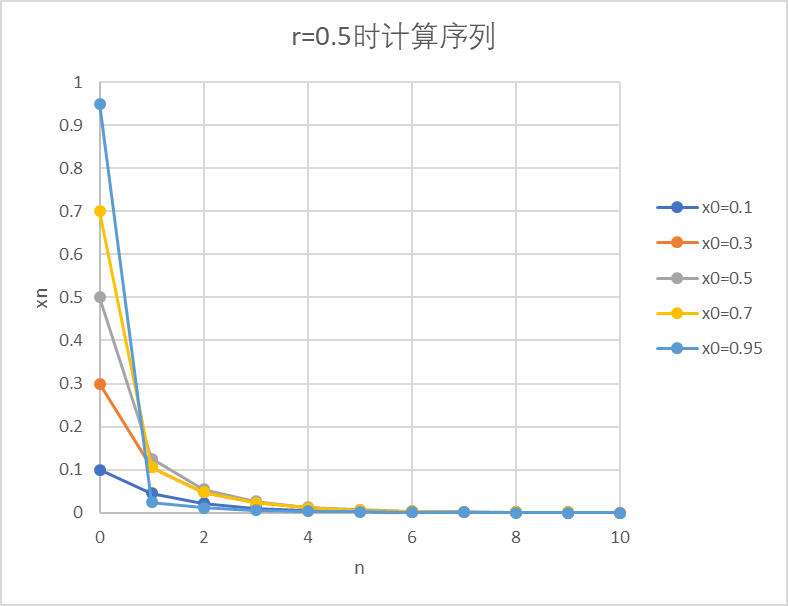
\includegraphics[width=0.6\textwidth]{r=0.5计算序列.png}
        \caption{r=0.5计算序列示意图}\label{r=0.5计算序列示意图}
    \end{figure}

    可以看出,无关于初值选取,序列收敛于0。并且观察到,关于0.5对称的两个点第一次迭代后序列完全相同(0.3和0.7),
    这可以通过下面迭代关系中右式关于0.5的对称性解释。
    \begin{equation}
        x_{n+1}=rx_n(1-x_n)
    \end{equation}

    r=1.5时,计算序列如下。

    % Table generated by Excel2LaTeX from sheet 'Sheet1'
    \begin{table}[H]
        \centering
        \caption{r=1.5计算序列数据表}
        \begin{tabular}{|c|c|c|c|c|c|}\hline
        \diagbox{n}{$x_0$}    & 0.1   & 0.3   & 0.5   & 0.7   & 0.95 \\\hline
        1     & 0.135000 & 0.315000 & 0.375000 & 0.315000 & 0.071250 \\\hline
        2     & 0.175163 & 0.323662 & 0.351563 & 0.323663 & 0.099260 \\\hline
        3     & 0.216721 & 0.328358 & 0.341949 & 0.328358 & 0.134111 \\\hline
        4     & 0.254629 & 0.330808 & 0.337530 & 0.330808 & 0.174188 \\\hline
        5     & 0.284690 & 0.332061 & 0.335405 & 0.332061 & 0.215770 \\\hline
        6     & 0.305462 & 0.332695 & 0.334363 & 0.332695 & 0.253820 \\\hline
        7     & 0.318233 & 0.333013 & 0.333847 & 0.333013 & 0.284093 \\\hline
        8     & 0.325441 & 0.333173 & 0.333590 & 0.333173 & 0.305076 \\\hline
        9     & 0.329294 & 0.333253 & 0.333461 & 0.333253 & 0.318007 \\\hline
        10    & 0.331289 & 0.333293 & 0.333397 & 0.333293 & 0.325318 \\\hline
        11    & 0.332305 & 0.333313 & 0.333365 & 0.333313 & 0.329229 \\\hline
        12    & 0.332818 & 0.333323 & 0.333349 & 0.333323 & 0.331256 \\\hline
        13    & 0.333075 & 0.333328 & 0.333341 & 0.333328 & 0.332288 \\\hline
        14    & 0.333204 & 0.333331 & 0.333337 & 0.333331 & 0.332809 \\\hline
        15    & 0.333269 & 0.333332 & 0.333335 & 0.333332 & 0.333071 \\\hline
        16    & 0.333301 & 0.333333 & 0.333334 & 0.333333 & 0.333202 \\\hline
        17    & 0.333317 & 0.333333 & 0.333334 & 0.333333 & 0.333268 \\\hline
        18    & 0.333325 & 0.333333 & 0.333334 & 0.333333 & 0.333300 \\\hline
        19    & 0.333329 & 0.333333 & 0.333333 & 0.333333 & 0.333317 \\\hline
        \end{tabular}%
        \label{r=1.5计算序列数据表}%
    \end{table}%
    
    绘图如下。
    \begin{figure}[H]
        \centering
        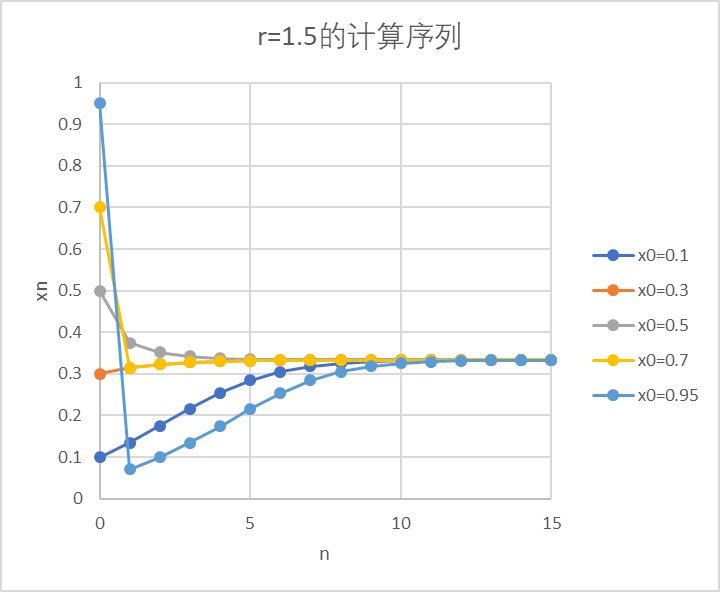
\includegraphics[width=0.6\textwidth]{r=1.5时计算序列.png}
        \caption{r=1.5计算序列示意图}\label{r=1.5计算序列示意图}
    \end{figure}

    可以看出,无关于初值选取,序列收敛于1/3。同样观察到,关于0.5对称的两个点第一次迭代后序列完全相同(0.3和0.7),
    这可以通过迭代关系中右式关于0.5的对称性解释。

    \textbf{本题源代码见附录。}

    \subsection{第2问}

    $x^*=f(x^*)=rx^*(1-x^*)$存在两个根
    \begin{align}
        x_1=0&&x_2=1-\frac{1}{r}
    \end{align}

    当$0<r\le 1$时,$x_2\le 0$;根据迭代关系,由于初值是(0,1)的正数,那么计算序列是正项序列(x>0,1-x>0),
    极限非负,所以不动点为0.

    当1<r<3时,$x_2>0$,下面将会证明,序列一定不收敛于0,于是不动点为$x_2$.(r<3将在第三问中说明)

    整理得到结论:

    $$x^*=
    \begin{cases}
    0& 0<x\le 1\\
    1-\frac{1}{r}& \text{1<x<3}
    \end{cases}$$
   
    绘图如下:

    \begin{figure}[H]
        \centering
        \includegraphics[width=0.6\textwidth]{x-r图1.jpg}
        \caption{x-r图1}\label{x-r图1}
    \end{figure}

    下面证明,1<r<3时序列不收敛于0.
    
    假设序列收敛于0,那么有

    \begin{align}
        \forall \epsilon \in (0,\frac{r-1}{2r}),\exists N>0,s.t.\forall n>N,0<x_n<\epsilon 
    \end{align}

    这时,
    
    \begin{align}
        x_{n+1}-x_n&=rx_n(1-x_n)-x_n\\
        &=rx_n(\frac{r-1}{r}-x_n)>0
    \end{align}

    于是n>N之后,{$x_n$}单增。又由于$ \lim_{n \to \infty} x_n=0 $,于是有$x_n\le0,\forall n>N$,
    与$x_n>0$矛盾,假设不成立。证毕。

    在本题中有

    \begin{align}
        \epsilon_{n+1}&=f'(x^*)\epsilon_n+\frac{1}{2}f''(x^*)\epsilon_n^2+\dots\\
        f'(x^*)&=r(1-2x^*)\\
        f''(x^*)&=-2r
    \end{align}

    于是,

    \begin{align}
        \lim_{n \to \infty} |\frac{\epsilon_{n+1}}{\epsilon_n}|=f'(x^*)=
        \begin{cases}
            r& 0<r\le1\\
            |2-r|&1<r<3
        \end{cases} 
    \end{align}

    其中,若r=2,有

    \begin{align}
        \lim_{n \to \infty} |\frac{\epsilon_{n+1}}{\epsilon_n^2}|=\frac{1}{2}f''(x^*)=r
    \end{align}

    根据收敛阶和收敛率的定义,

    \begin{align}
        0&<r\le1 & p&=1 & C&=r\\
        1&<r<3(r\neq 2)  & p&=1 & C&=2-r\\
        r&=2 & p&=2 & C&=r
    \end{align}

    \subsection{第3问}

    r>3时,数列将无法收敛,因为$\lim_{n \to \infty}\frac{\epsilon_{n+1}}{\epsilon_n}=|2-r|>1$.

    取r=3.1,计算序列原始数据见文件$“question3\_data.txt”$。

    绘得下图

    \begin{figure}[H]
        \centering
        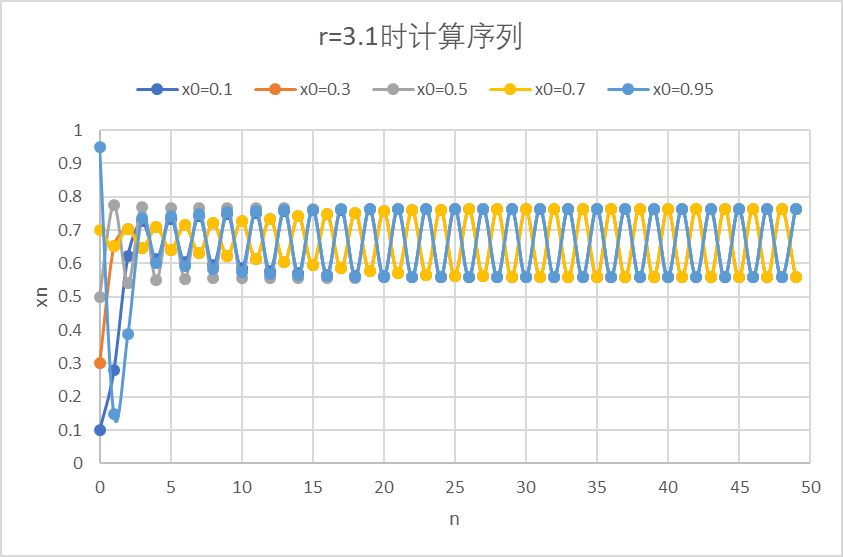
\includegraphics[width=0.6\textwidth]{r=3.1时计算序列.png}
        \caption{r=3.1计算序列示意图}\label{r=3.1计算序列示意图}
    \end{figure}

    由图可知,无论初值如何选取,序列将在两个值之间来回振荡。

    
    \subsection{第4问}

    先证明收敛条件。

    根据迭代关系式$x_{n+2}=f(f(x_n))$,误差的泰勒展开式为

    \begin{align}
        \epsilon_{n+2}&=\frac{d}{dx}f(f(x_i^*))\epsilon_n+\frac{1}{2}\frac{d^2}{dx^2}f(f(x_i^*))\epsilon_n^2+\dots
    \end{align}
    
    其中,$x_i^*(i=1,2)$是序列收敛到的两个值。并且有关系$f(x_1^*)=x_2^*,f(x_2^*)=x_1^*$。

    于是,
    
    \begin{align}
        lim_{n\to\infty}|\frac{\epsilon_{n+1}}{\epsilon_n}|=|\frac{d}{dx}f(f(x_i^*))|=|f'(x_i^*)f'(x_j^*)|=|f'(x_1^*)f'(x_2^*)|
    \end{align}

    序列收敛,因而一定有$|f'(x_1^*)f'(x_2^*)|\le1$。证毕。

    根据$f(f(x^*))=x^*$,解得
    
    \begin{align}
        x_1&=0 & x_2&=1-\frac{1}{r} & x_3&=\frac{r^2+r+\sqrt{r^2(r+1)(r-3)}}{2r^2} & x_4&=\frac{r^2+r-\sqrt{r^2(r+1)(r-3)}}{2r^2}
    \end{align}

    其中,$x_1,x_2$为单次迭代稳定解,舍去,$x_3,x_4$才是我们想要的$x_1^*,x_2^*$。进一步,为确定r的取值范围,代入必要条件$|f'(x_1^*)f'(x_2^*)|\le1$,
    获得正区间解集$3<r<3.44949$。

    在图\ref{x-r图1}中补充后绘得下图。

    \begin{figure}[H]
        \centering
        \includegraphics[width=0.6\textwidth]{x-r图2.jpg}
        \caption{x-r图2}\label{x-r图2}
    \end{figure}

    \subsection{第5问}
    \subsubsection{周期四和八展示}
    选取r=3.5,发现周期为4,迭代100000次后展示如下。

    \begin{figure}[H]
        \centering
        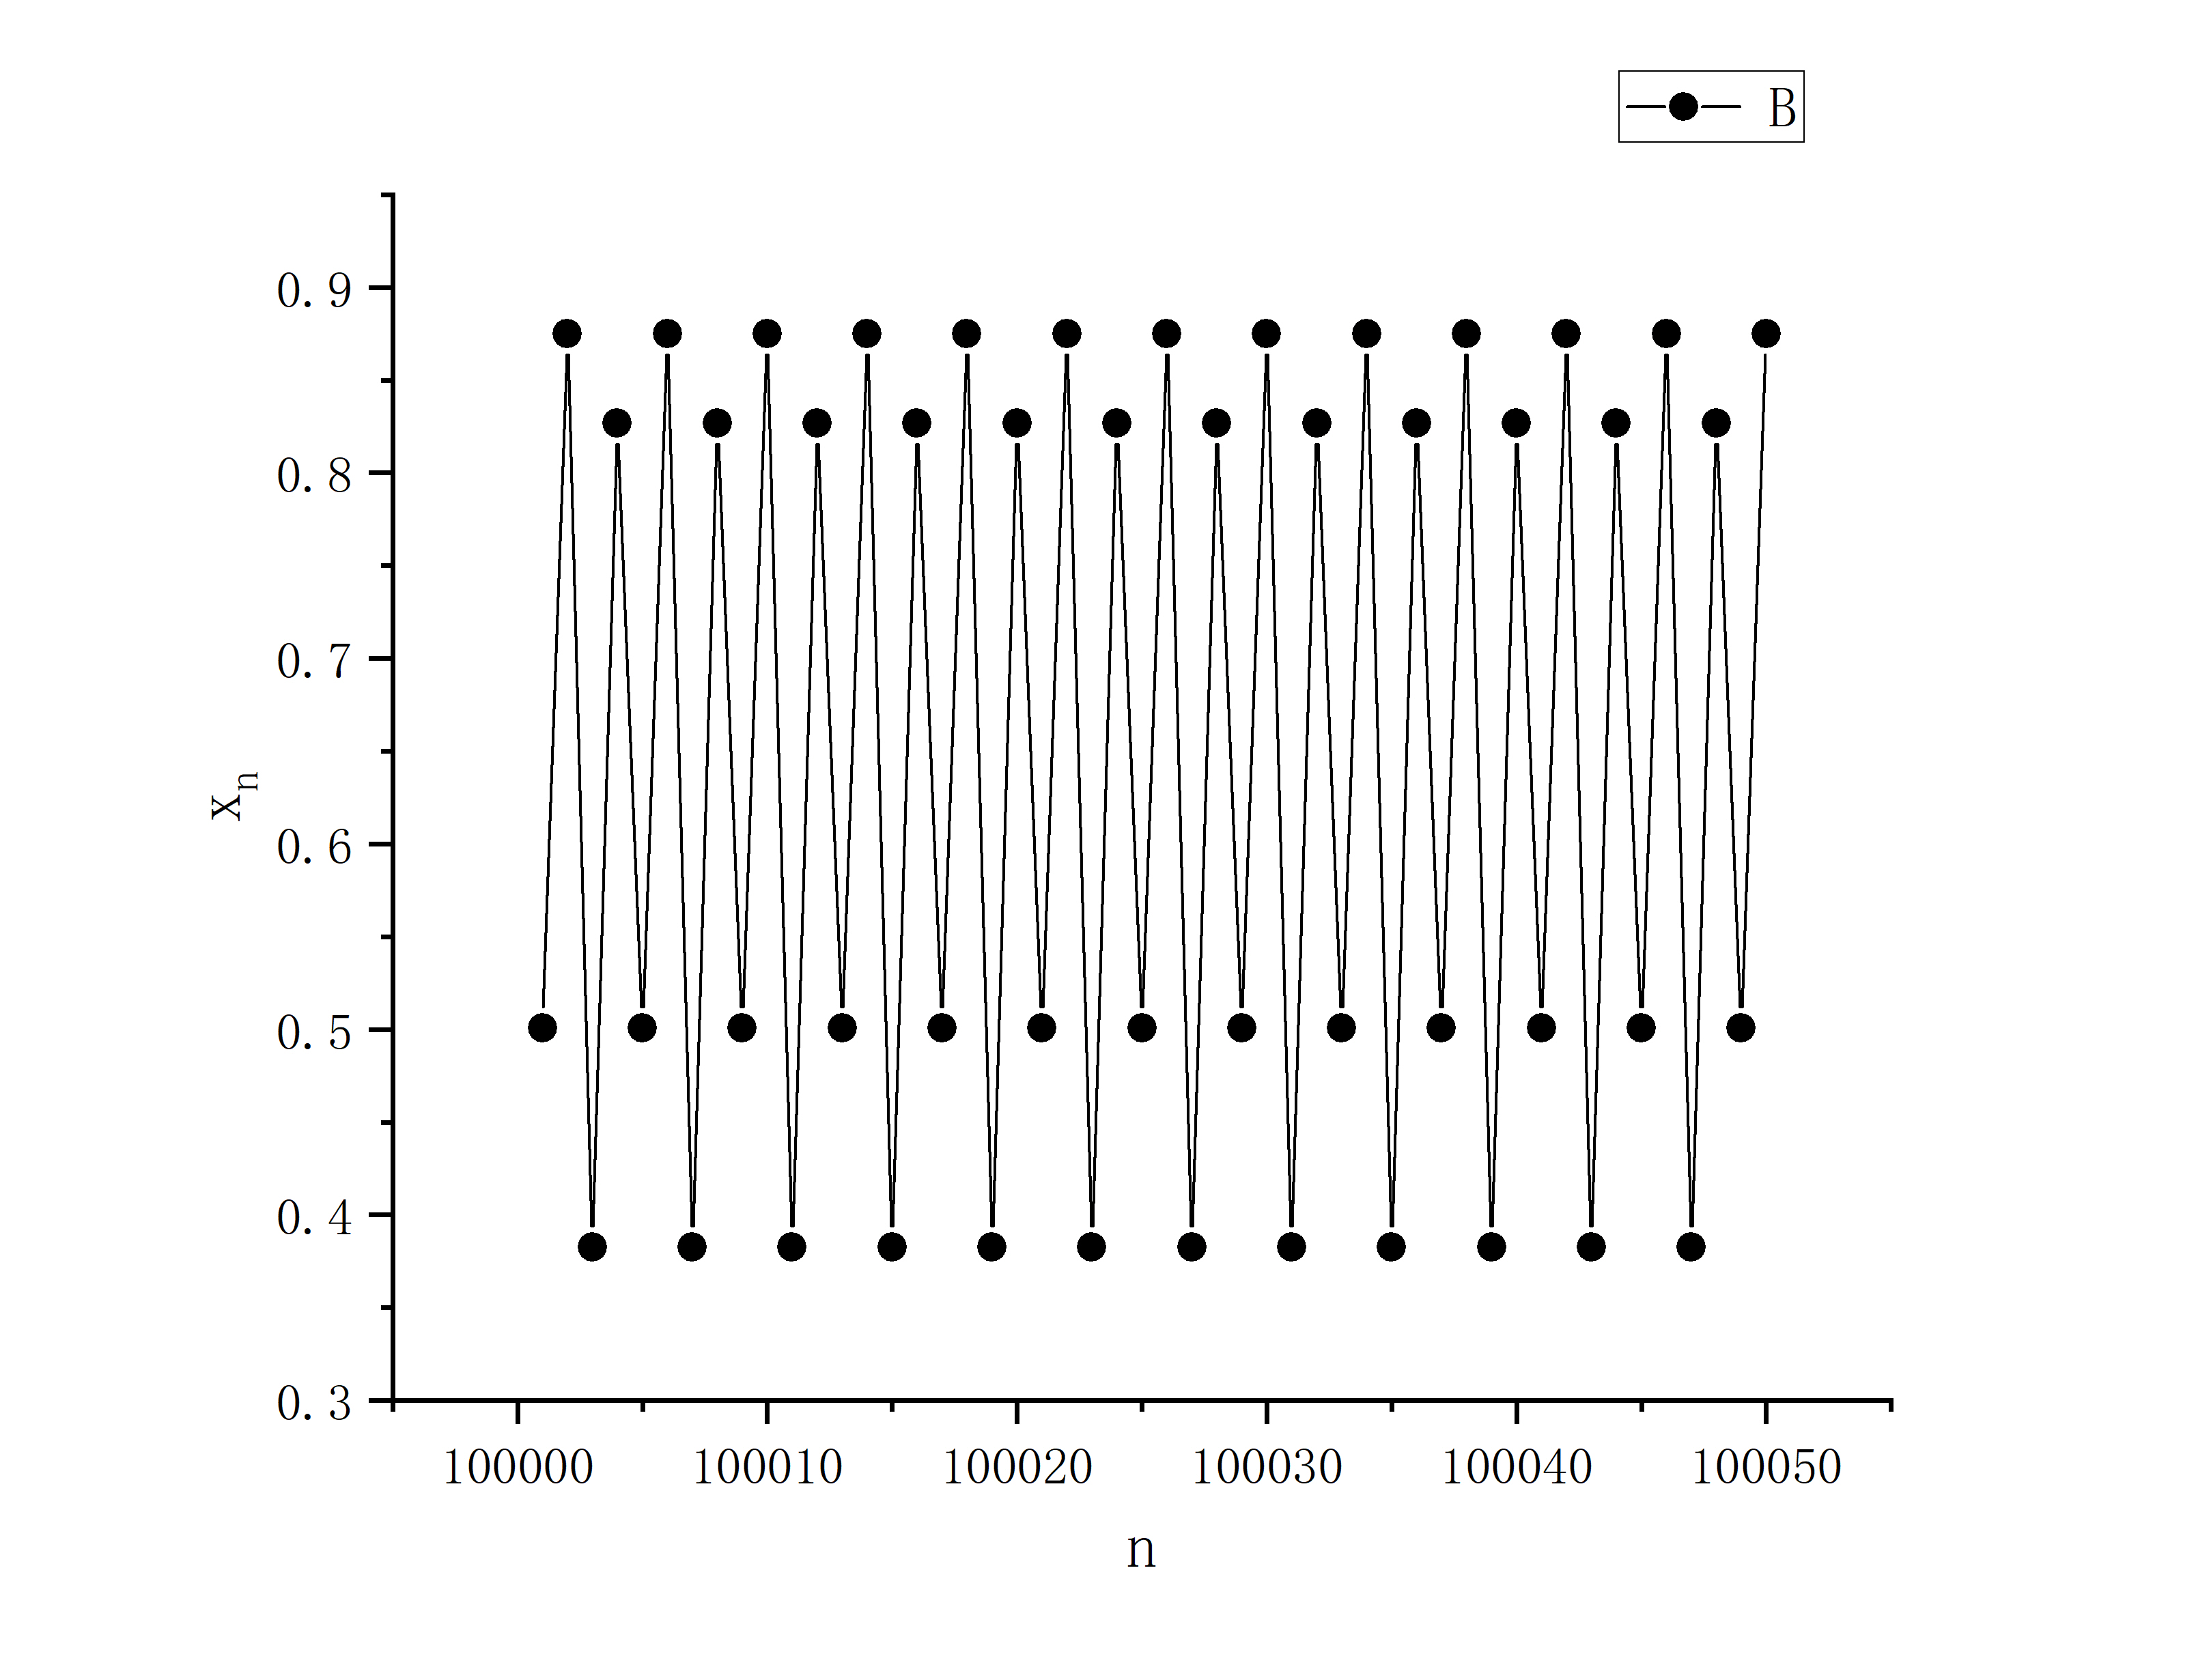
\includegraphics[width=0.6\textwidth]{周期四展示(r=3.5).jpg}
        \caption{周期四展示(r=3.5)}\label{周期四展示(r=3.5)}
    \end{figure}

    选取r=3.55,发现周期为8,迭代100000次后展示如下。

    \begin{figure}[H]
        \centering
        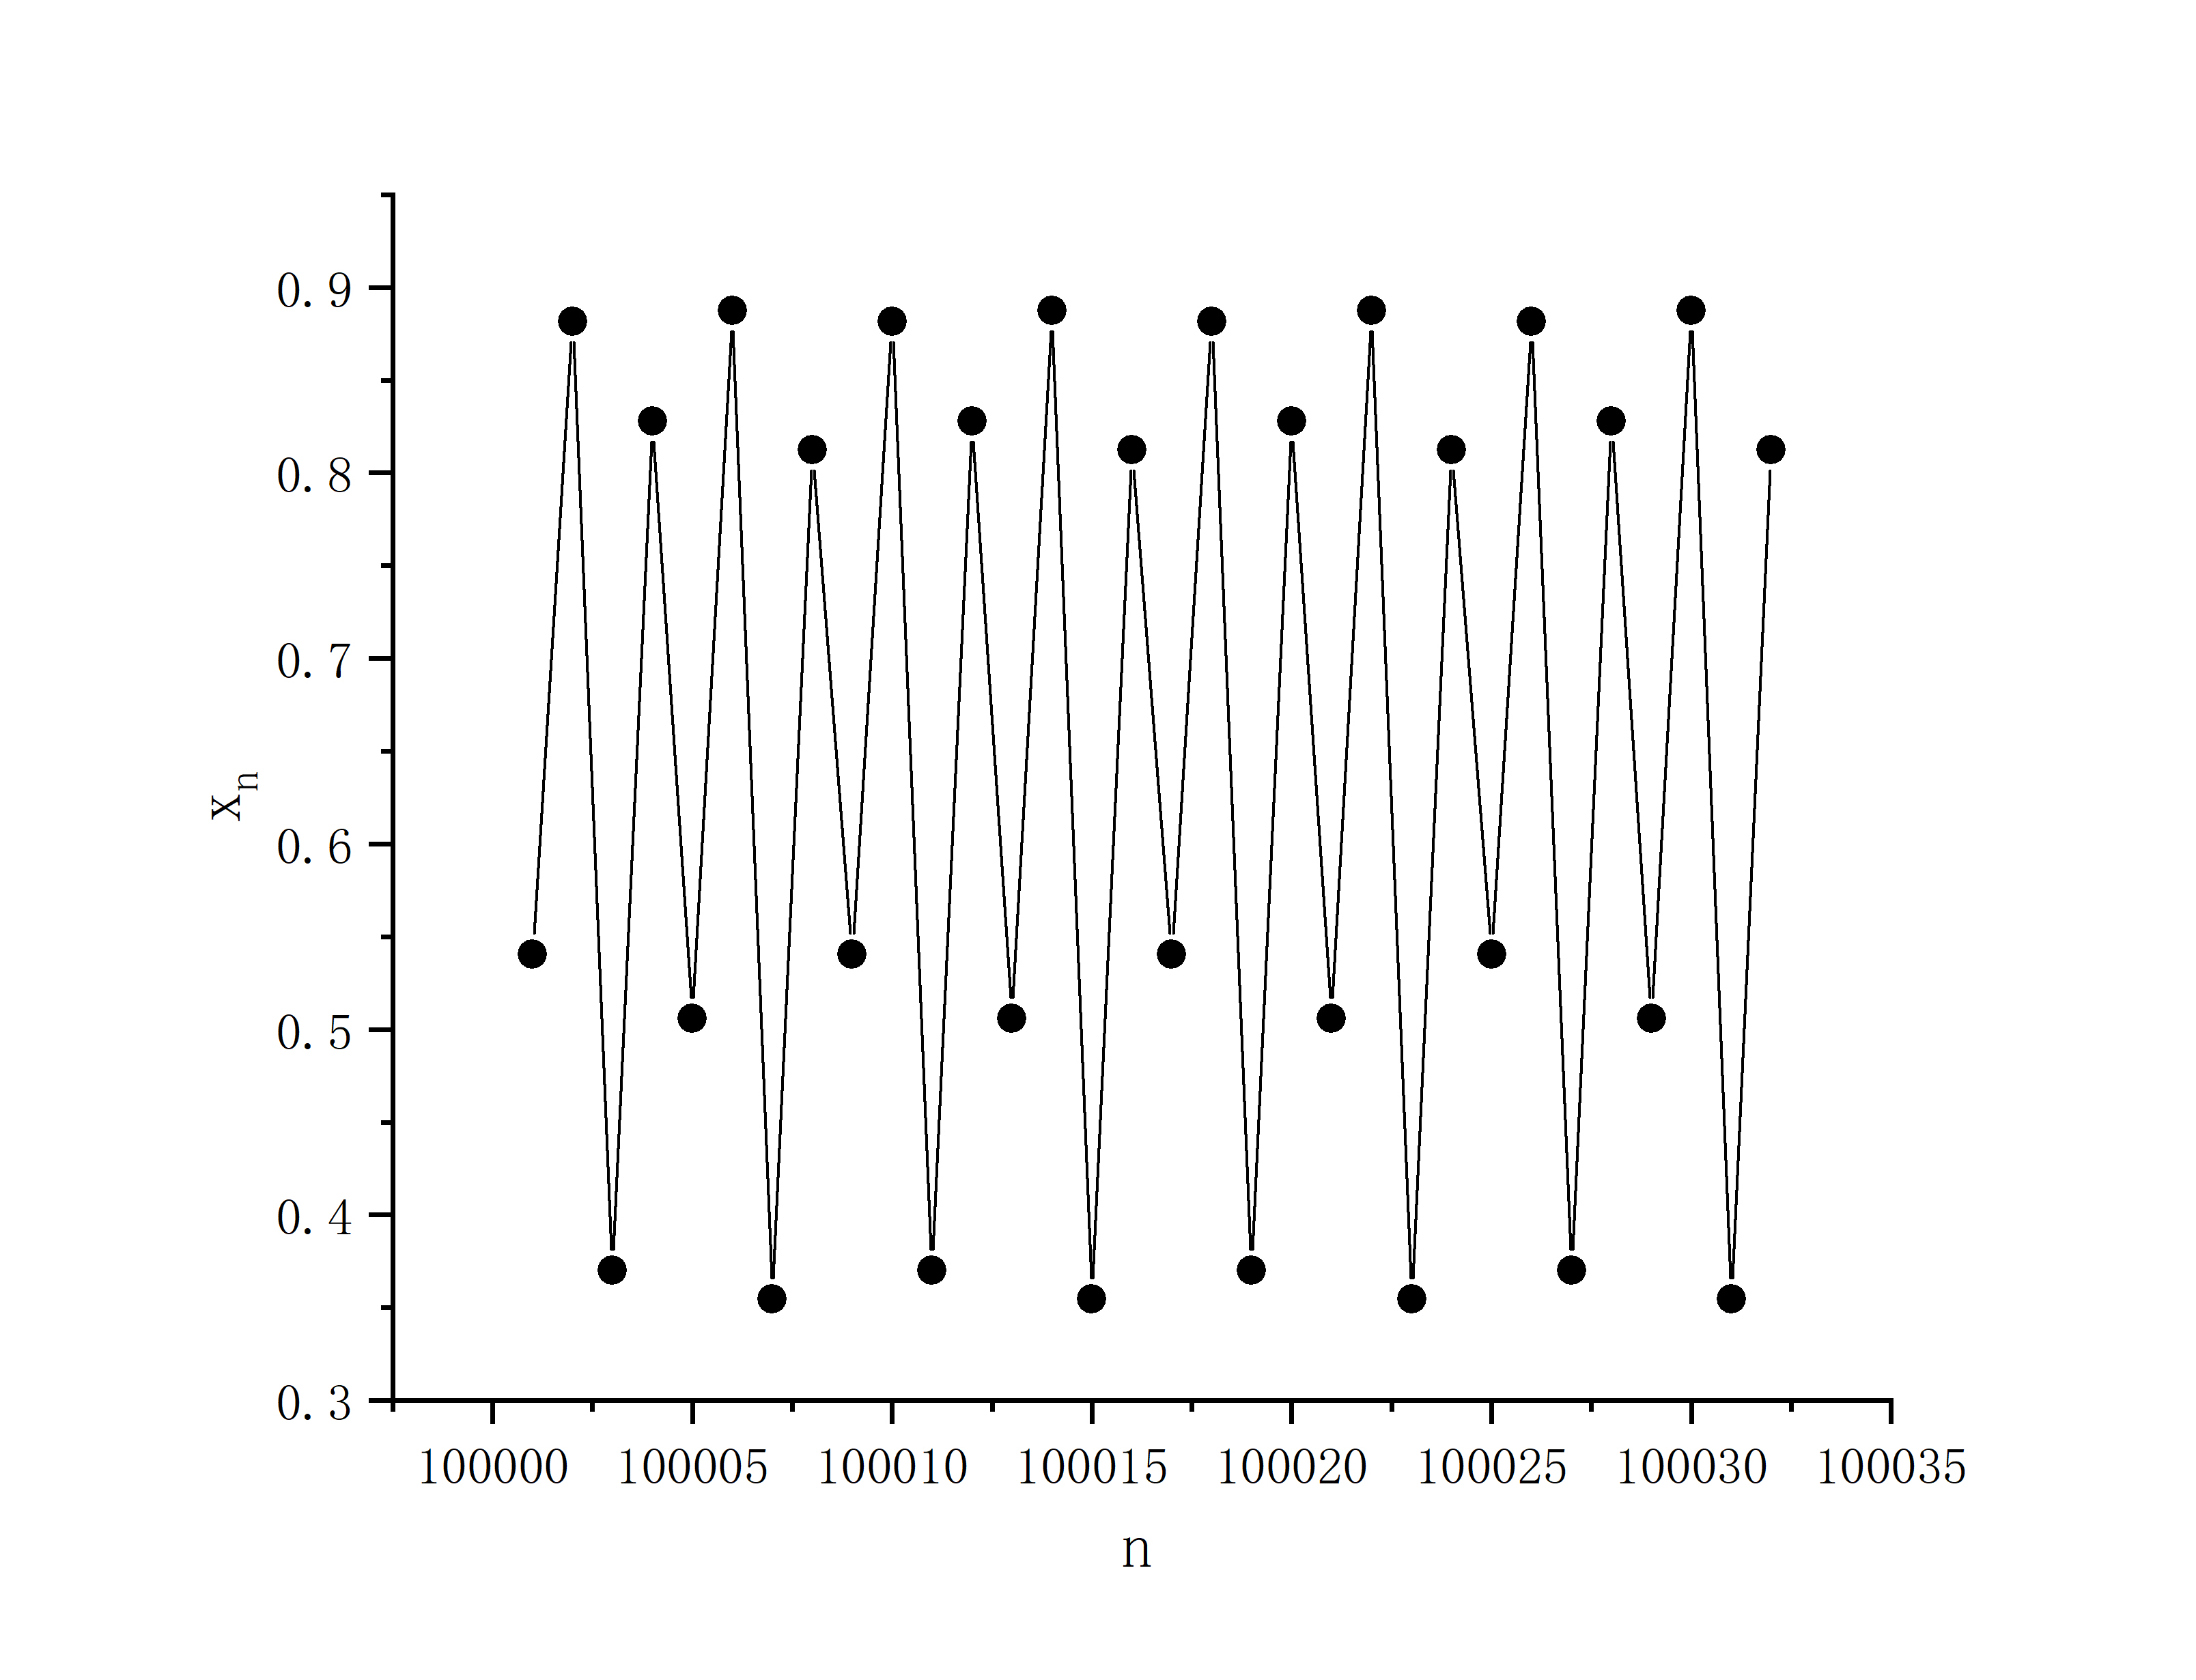
\includegraphics[width=0.6\textwidth]{周期八展示(r=3.55).jpg}
        \caption{周期八展示(r=3.55)}\label{周期八展示(r=3.55)}
    \end{figure}

    代码实现类似第一问代码,具体见附录。

    \subsubsection{r>3时周期数随r变化关系的初步探索}

    为对周期变化趋势有一个更加细致的了解,作者尝试不同的r(r>3)试着输出迭代次数充分多后的序列,并观察周期性特征,初步得到如下结论。

    \begin{align*}
        3&<r\le 3.4494 & &\text{周期为2}\\
        3.4495&\le r \le 3.5440 & &\text{周期为4}\\
        3.5441&\le r \le 3.5644 & &\text{周期为8}\\
        3.5645&\le r \le 3.5687 & &\text{周期为16}\\
        3.5688&\le r \le 3.5696 & &\text{周期为32}\\
        3.5697&\le r \le 3.5698 & &\text{周期为64}\\
        3.5699&\le r \le 3.56993 & &\text{周期为128}\\
        &r\ge3.57 & &\text{无明显周期}
    \end{align*}

    从上述结论中也可以得到每个周期变化的分点的大致位置:

    \begin{align*}
        3.4494&< r < 3.4495 & &\text{出现周期2和4的分点}\\
        3.5440&< r < 3.5441 & &\text{出现周期4和8的分点}\\
        3.5644&< r < 3.5645 & &\text{出现周期8和16的分点}\\
        3.5687&< r < 3.5688 & &\text{出现周期16和32的分点}\\
        3.5696&< r < 3.5697 & &\text{出现周期32和64的分点}\\
        3.5698&< r < 3.5699 & &\text{出现周期64和128的分点}\\
    \end{align*}\label{分点估计}

    \subsubsection{收敛速度的定义}

    \paragraph{周期为1的情况}

    不失一般性,我们先讨论单值收敛的情况。

    给出如下定义:

    \begin{definition}\label{def1}
        给定一个实数序列${x_n}$,满足迭代关系$x_{n+1}=f(x_n)$,并且$\lim_{n\to\infty}x_n=\alpha$。如果f在定义域内一阶导数连续,
        且$f'(\alpha)\neq 0$,那么${x_n}$的收敛速度V定义为$\frac{1}{f'(\alpha)}$。
    \end{definition}
    
    回顾收敛阶和收敛率的定义,这个收敛速度就是一阶收敛率$C_1$的倒数。由于收敛序列满足$0\le C_1\le 1$,且越靠近0收敛速度越快。
    因此对于收敛速度V,有收敛序列满足$1\le V \le \infty$,且V越大收敛速度越快。

    下面面临数值计算V的问题。如果按照定义,需要数值求出极限值$\alpha$,再代回$1/f'(x)$中。这样就需要解析的求$f(x)$的导数,而且也需要一个比较精确的极限值。
    可是,能否不求出极限值、不求导数就能数值计算出收敛速度呢?作者下面提出一种方法。

    首先证明一个定理。

    \begin{theorem}\label{thm1}
        实数序列${x_n}$满足迭代关系$x_{n+1}=f(x_n)$,并且$\lim_{n\to\infty}x_n=\alpha$。如果f在定义域内一阶导数连续,
        且$f'(\alpha)\neq 0$,那么
        \begin{equation*}
            \lim_{n \to \infty}\frac{x_{n+1}-x_n}{x_{n+2}-x_{n+1}}=\frac{1}{f'(\alpha)}
        \end{equation*}
    \end{theorem}

    \begin{proof}\label{pf1}
        f(x)连续可微,应用第一中值定理有

        \begin{align*}
            x_{n+2}-x_{n+1}=f(x_{n+1})-f(x_n)=f'(\xi_n )(x_{n+1}-x_n),\exists\xi_n \in [x_n,x_{n+1}]
        \end{align*}

        故

        \begin{align*}
            \frac{x_{n+1}-x_n}{x_{n+2}-x_{n+1}}=\frac{1}{f'(\xi_n)}
        \end{align*}

        另知,$\lim_{n \to \infty}\xi_n=\alpha$(因为$\lim_{n \to \infty}x_n=\alpha,\lim_{n \to \infty}x_{n+1}=\alpha,x_n\le\xi_n\le x_{n+1}$)

        由f一阶导数连续,且$f'(\alpha)\neq 0$,故$\lim_{n \to \infty}\frac{1}{f'(\xi_{n})}=\frac{1}{f'(\alpha)}$

        \begin{equation*}
            \lim_{n \to \infty}\frac{x_{n+1}-x_n}{x_{n+2}-x_{n+1}}=\frac{1}{f'(\alpha)}
        \end{equation*}
        \end{proof}
        
        于是,根据定理\ref{thm1},我们可以计算序列$\{\frac{x_{n+1}-x_n}{x_{n+2}-x_{n+1}}\}$的极限值,即为收敛速度。

    \paragraph{周期为N的情况}

    设序列N个收敛点为$\alpha_1,\alpha_2,\dots ,\alpha_N$,并且满足$\alpha_{i+1}=f(\alpha_i)(i=1,2,\dots,N-1),\alpha_1=f(\alpha_N)$。
    且$\alpha_1,\alpha_2,\dots ,\alpha_N$一定是方程$\overbrace{f(f(\dots f}^{N\text{个}}(x)\dots))=x$的解。

    由于数列的周期性,子序列{$x_{n_k}$}($n_k=i+8k,i=1,2,\dots,N$)一定是收敛子序列,不妨设收敛点为$\alpha_i$。

    我们已经讨论过单值收敛的情形,可以将定义\ref{def1}应用到子序列上,并且根据定理\ref{thm1}计算序列$\{\frac{x_{n_{k+1}}-x_{n_k}}{x_{n_{k+2}}-x_{n_{k+1}}}\}$
    的极限值,就得到子序列的收敛速度。

    那么问题来了,每一个子序列我们都能得到一个收敛速度,那么该怎样用这N个收敛速度描述整个序列的收敛速度呢?事实上,我们下面证明,每一个子序列的收敛速度相同,
    
    易知,每个子序列满足递推关系:$x_{n_{k+1}}=\overbrace{f(f(\dots f}^{N\text{个}}(x_{n_k})\dots))$,根据定义\ref{def1},
    子序列的收敛速度
    
    \begin{align}
        V_i=\frac{1}{\frac{d}{dx}\overbrace{f(f(\dots f}^{N\text{个}}(\alpha_i)\dots))}=\frac{1}{f'(\alpha_1)f'(\alpha_2)\dots f'(\alpha_N)}
    \end{align}\label{每个子序列收敛速度一样}
    
    可见,每个子序列收敛速度一样,进而我们可以任意选用其中一个代表整个序列的收敛速度。

    于是,我们不难将定义\ref{def1}和定理\ref{thm1}推广到周期为N的情形。

    \begin{definition}\label{def2}
        给定一个实数序列${x_n}$,满足迭代关系$x_{n+1}=f(x_n)$,并且在$n \to \infty$时数列化为周期为N的稳定震荡,
        N个稳定值为$\alpha_1,\alpha_2,\dots ,\alpha_N$。如果f在定义域内一阶导数连续,
        且$f'(\alpha_i)\neq 0(i=1,2,\dots,N)$,那么${x_n}$的收敛速度V定义为$\frac{1}{f'(\alpha_1)f'(\alpha_2)\dots f'(\alpha_N)}$。
    \end{definition}

    \begin{theorem}\label{thm2}
        实数序列${x_n}$满足迭代关系$x_{n+1}=f(x_n)$,并且在$n \to \infty$时数列化为周期为N的稳定震荡,
        N个稳定值为$\alpha_1,\alpha_2,\dots ,\alpha_N$。如果f在定义域内一阶导数连续,
        且$f'(\alpha_i)\neq 0(i=1,2,\dots,N)$,那么
        \begin{equation*}
            \lim_{n \to \infty}\frac{x_{n+N}-x_n}{x_{n+2N}-x_{n+N}}=\frac{1}{f'(\alpha)}
        \end{equation*}
    \end{theorem}

    于是,对于周期为N的序列,我们只需计算数列$\{\frac{x_{n+N}-x_n}{x_{n+2N}-x_{n+N}}\}$的极限值即可。

    \subsubsection{二分法求解周期分点的精确值}

    题目要求画出收敛速度随r的变化图像,我们需要细分区间,选定不同的r,计算收敛速度,并描点作图。但是对于给定的r,需要我们提前确定振荡周期N。
    由于我们需要对r作细致的细分,我们需要知道周期随r变化关系更加细致的了解。由于我们已经确定周期分点到小数点后4位(见\ref{分点估计}节),我们利用它
    并利用二分法原理,进一步提高分点的有效数字位数。

    我们需要编写一个程序,在给定区间有一个周期分点,分点左边是一个周期,分点右边是另一个周期,我们需要数值求出这个分点。这容易让我们联想到
    二分求根,用类似的方法,我们可以写出这个算法。

    \begin{algorithm}[H]  
        \caption{ 二分法求解周期分点的值}  
        \label{二分法求解周期分点的精确值}  
        \begin{algorithmic}[1]  
        \Require  
            区间左端点A,A处周期数N,区间右端点B(B处周期数为2N)  
        \Ensure  
            周期变化分点的值(精确到给定精度EPS1)
        \If {A处周期不为N或B处周期不为2N}
            \State 报错
        \EndIf
                    
        \State m=(A+B)/2 \label{迭代起点} 
        
        \If {m处周期为N}
            \State A=m
        \Else
            \State B=m
        \EndIf\label{迭代终点}

        \If {|A-B|<EPS1}
            \State 重复\ref{迭代起点}-\ref{迭代终点}
        \Else
            \State 输出 (A+B)/2
        \EndIf
        \end{algorithmic}  
      \end{algorithm}  

    具体代码实现见附录。这个算法需要手动输入周期分点的粗略区间,但是好处是可以设置精度,进而可以精确到很多位数。
    下面给出用这个程序计算分点的输入输出。

    % Table generated by Excel2LaTeX from sheet 'Sheet6'
    \begin{table}[H]
        \centering
        \caption{二分法计算分点输入输出表格}
        \begin{tabular}{|c|c|c|c|}\hline
        A     & B     & N     & OUTPUT \\\hline
        2     & 3.2   & 1     & 2.9999990082 \\\hline
        3.4494 & 3.4495 & 2     & 3.4494890324 \\\hline
        3.5440 & 3.5441 & 4     & 3.5440900577 \\\hline
        3.5644 & 3.5645 & 8     & 3.5644071382 \\\hline
        3.5687 & 3.5688 & 16    & 3.5687593623 \\\hline
        3.5696 & 3.5697 & 32    & 3.5696916032 \\\hline
        3.5698 & 3.5699 & 64    & 3.5698912557 \\\hline
        3.5699 & 3.5699 & 128   & 3.5699340160 \\\hline
        3.56994 & 3.569945 & 256   & 3.5699431750 \\\hline
        3.569945 & 3.5699452 & 512   & 3.5699451371 \\\hline
        \end{tabular}%
        \label{二分法计算分点输入输出表格}%
    \end{table}%
    
    \subsubsection{绘制V-r图}

    由于r>3.57时序列出现混沌现象,无法定义收敛速度,下面我们只考虑0<r<3.569892情况,这时周期小于等于64。

    在[0.0001,3.569891]上等间隔取点,间隔设置为0.00001,根据表\ref{二分法计算分点输入输出表格}判断每个r值对应的周期数N,
    计算序列$\{\frac{x_{n+N}-x_n}{x_{n+2N}-x_{n+N}}\}$的极限值,即为收敛速度。

    具体代码实现见附录。

    代码运行结果见$"convergentSpeed\_Data.txt"$

    根据输出结果绘制出散点图,其中,纵轴采用了对数标度(log10).

    \begin{figure}[H]
        \centering
        \includegraphics[width=0.8\textwidth]{V-r图.jpg}
        \caption{V-r图}\label{V-r图}
    \end{figure}

    标出四个极小值点如下图,对比表\ref{二分法计算分点输入输出表格},正是周期分点所在的位置。

    \begin{figure}[H]
        \centering
        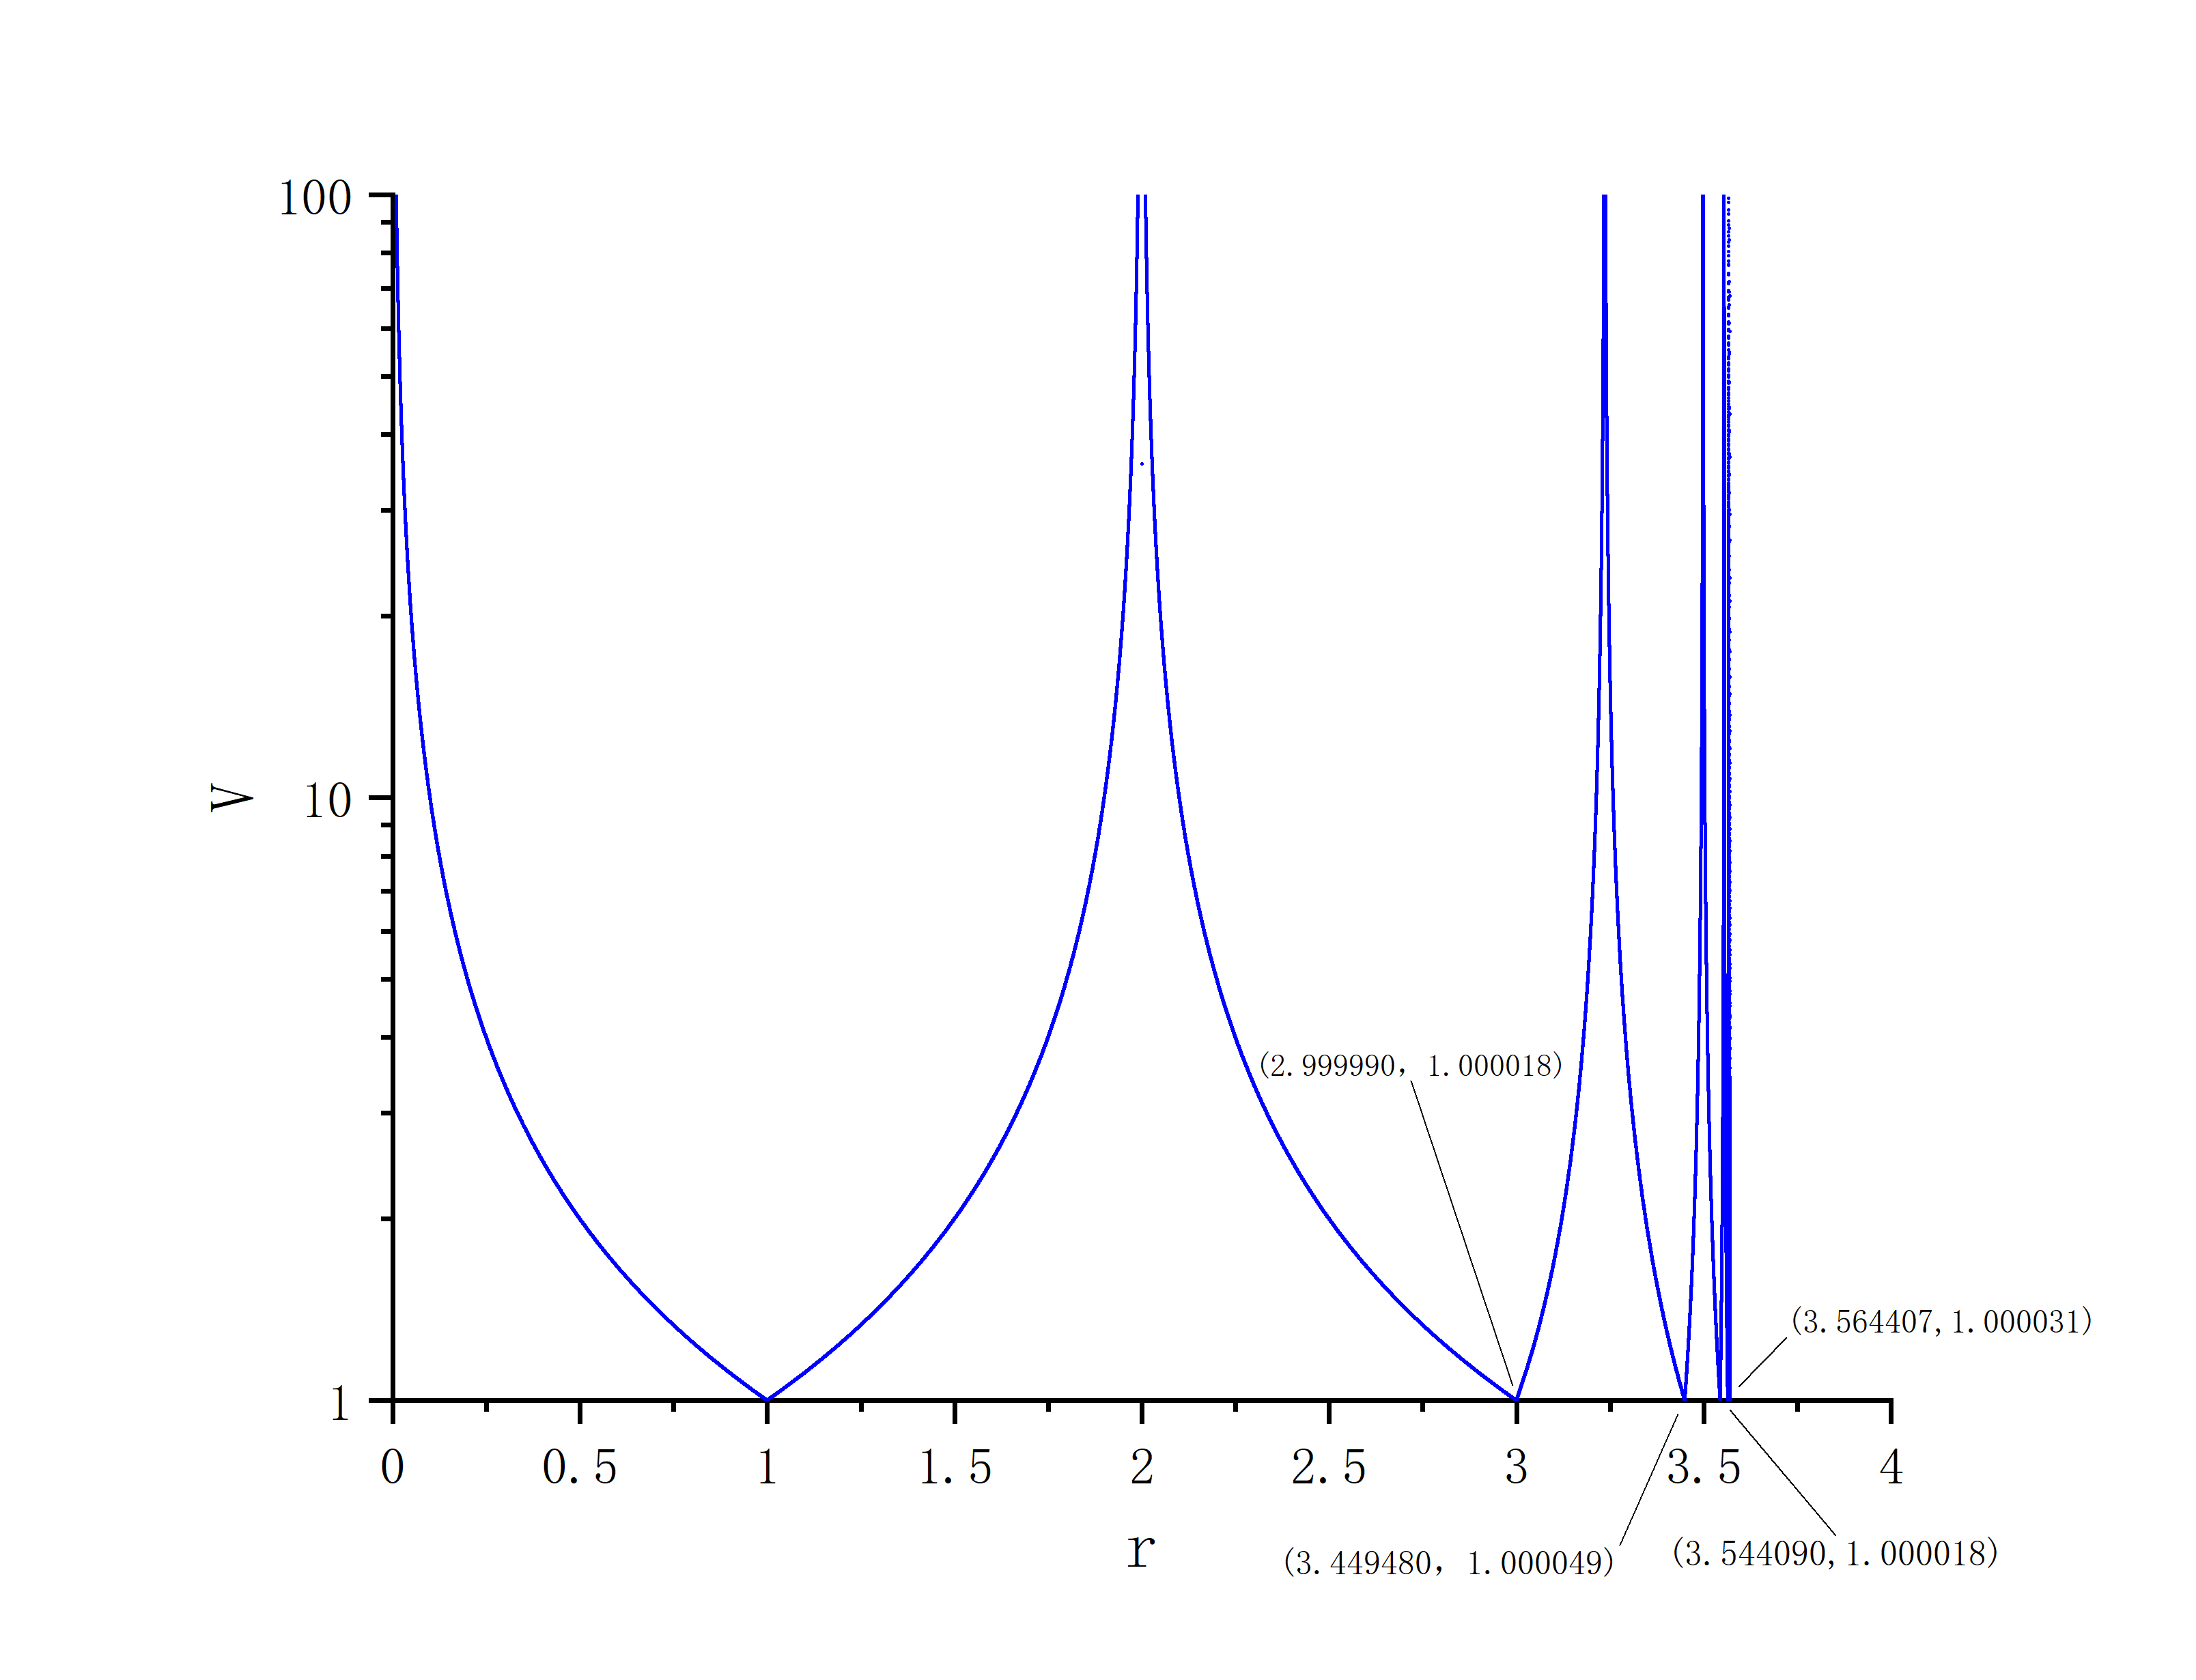
\includegraphics[width=0.8\textwidth]{V-r图(标记分点).jpg}
        \caption{V-r图(标记分点)}\label{V-r图(标记分点)}
    \end{figure}

    可以得到结论,收敛速度为1是不同周期的分界点(r=1除外);在每个周期稳定的区间内,随着r的增大,收敛速度先增大后减小(周期为1除外)。
    
    \subsection{第6问}

    本问需要绘制$x^*-r$关系,作者采取细分区间、数值计算$x^*$的方式再描点作图的方式作出。

    如何得到$x^*$呢?我们通过不断迭代找到稳定收敛点。由于不同的r值收敛速度显著不同(图\ref{V-r图}),
    我们不能采用固定的很大的迭代次数。而且为了后面做出二分点、四分点的局域图,确定的迭代次数使得取点时收敛点顺序被打乱。
    因此我们采用监控子序列改变值的方法判断收敛与否。根据表\ref{二分法计算分点输入输出表格},我们在给定r值时知道收敛周期N。
    那么每次迭代N次,观察迭代前后的差值,小于精度EPS时认为收敛,然后输出这个点之后的N个值即可。

    具体代码实现见附录。

    代码运行结果见$"question6\_data.txt"$。

    做出散点图如下。

    \begin{figure}[H]
        \centering
        \includegraphics[width=0.6\textwidth]{x-r图3.jpg}
        \caption{x-r图3}\label{x-r图3}
    \end{figure}

    将坐标原点放到周期一和周期二的分界点得到。

    \begin{figure}[H]
        \centering
        \includegraphics[width=0.6\textwidth]{x-r图(magnify1-2).jpg}
        \caption{x-r图(magnify1-2)}\label{x-r图(magnify1-2)}
    \end{figure}

    将坐标原点放到周期二和周期四的分界点得到。

    \begin{figure}[H]
        \centering
        \includegraphics[width=0.8\textwidth]{x-r图(magnify2-4).jpg}
        \caption{x-r图(magnify2-4)}
        \label{fig:x-r-magnify2-4}
    \end{figure}

    将坐标原点放到周期四和周期八的分界点得到。

    \begin{figure}[H]
        \centering
        \includegraphics[width=0.8\textwidth]{x-r图(magnify4-8).jpg}
        \caption{x-r图(magnify4-8)}
        \label{fig:x-r-magnify4-8}
    \end{figure}

    其中,在绘制图\ref{fig:x-r-magnify2-4}和图\ref{fig:x-r-magnify4-8}时,由于原始数据将r值一定的不同
    $x^*$打在一起,分开作图时需要将数据分离。作者分离数据时编写了两个小程序,请参考splitter文件夹。

    \subsection{第7问}

    将表\ref{二分法求解周期分点的精确值}周期分点相邻两项做差,并取自然对数,得到下表。

    % Table generated by Excel2LaTeX from sheet 'Sheet6'
    \begin{table}[H]
        \centering
        \caption{$\Delta r$数据表}
        \begin{tabular}{|c|c|}\hline
            $\Delta r$&$ln(\Delta r)$ \\\hline
        0.4494900242  & -0.799642 \\\hline
        0.0946010253  & -2.358087 \\\hline
        0.0203170805  & -3.896293 \\\hline
        0.0043522241  & -5.437068 \\\hline
        0.0009322409  & -6.977919 \\\hline
        0.0001996525  & -8.518932 \\\hline
        0.0000427603  & -10.05990 \\\hline
        0.0000091590  & -11.60077 \\\hline
        0.0000019621  & -13.14150 \\\hline
        \end{tabular}%
        \label{tab:Delta-r数据表}%
    \end{table}%
    
    将$ln(\Delta r)$与行数n作线性拟合,得到

    \begin{figure}[H]
        \centering
        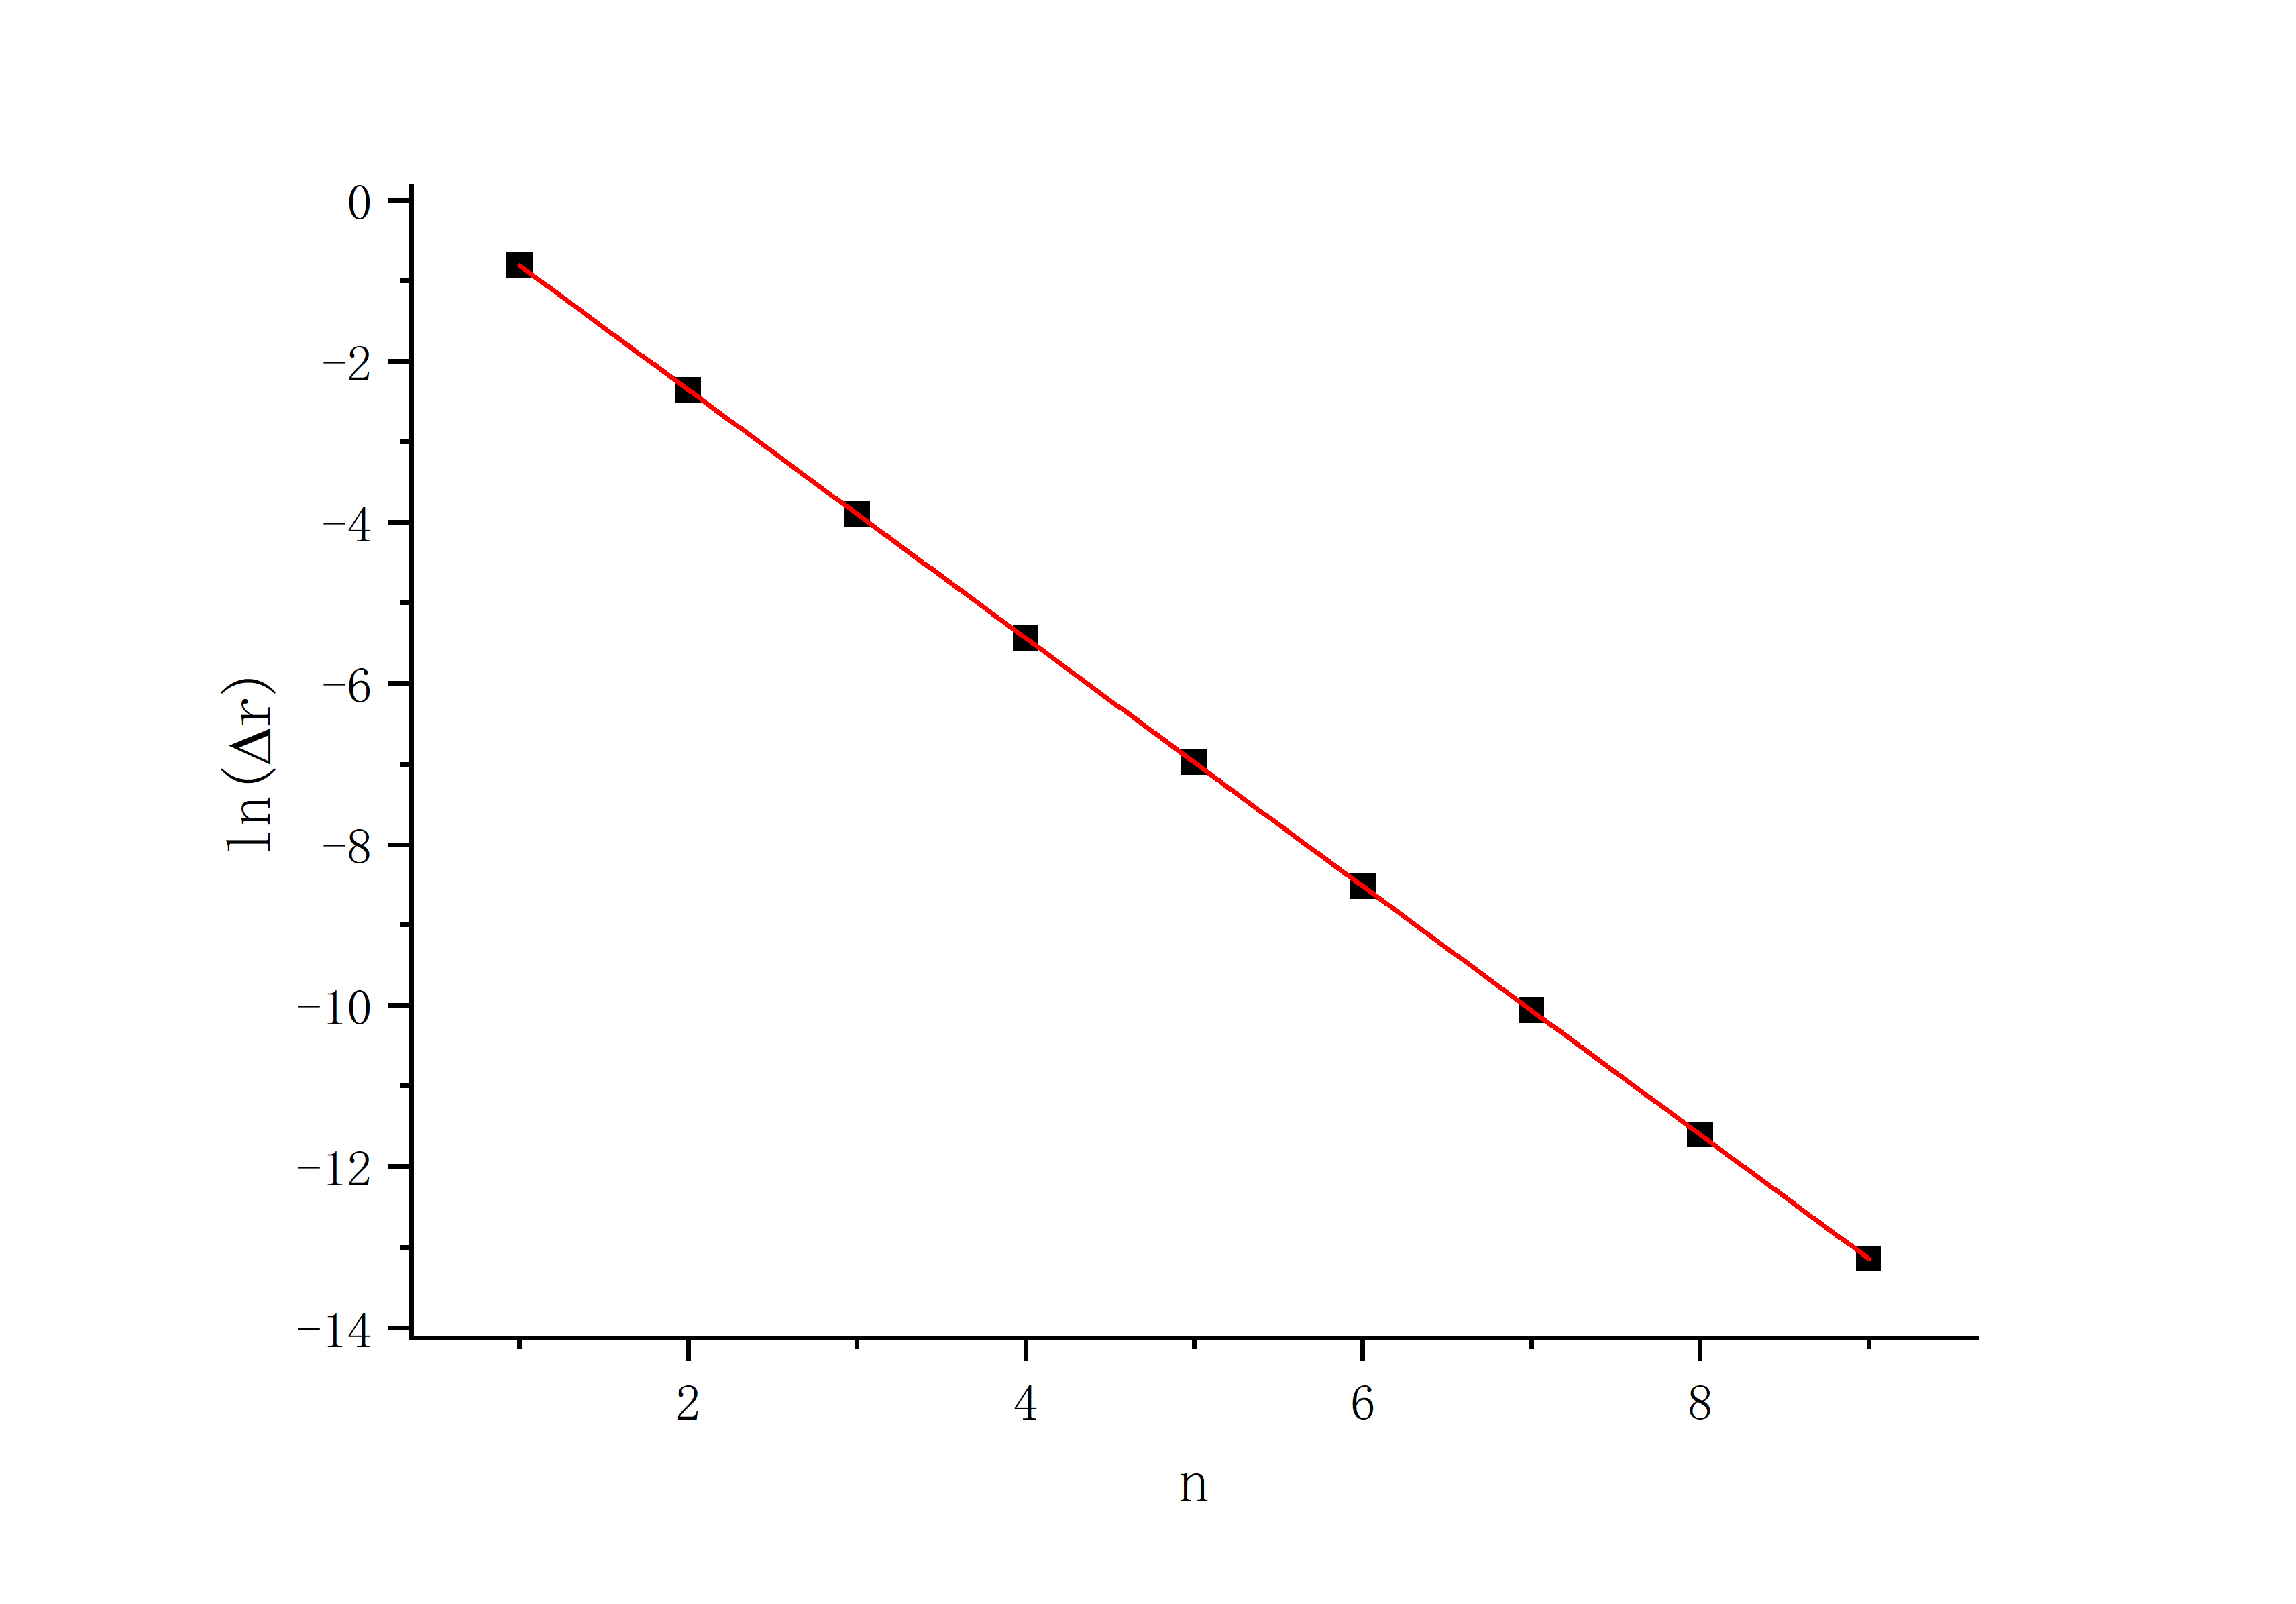
\includegraphics[width=0.6\textwidth]{r变化量趋势.jpg}
        \caption{r变化量趋势}
        \label{r变化量趋势}
    \end{figure}

    \begin{align}
        ln(\Delta r)&=k\cdot n+b\\
        k&=-1.54174\\
        b&=0.73203\\
        r&=0.9999994
    \end{align}

    于是,相邻两项$\Delta r$之比应为$F=e^k=0.214008$(后面一项比前面一项)。

    根据第一项$\Delta r_0=0.4494900242$得到$r_\infty$为

    \begin{align}
        r_\infty=3+\Delta r_0+\Delta r_0\cdot F+\Delta r_0\cdot F^2+\dots=3+\Delta r_0\cdot \frac{1}{1-F}=3.571876
    \end{align}

    这与我们在r>3.7看到的混沌现象基本一致。首先r>$r_\infty$一定是混沌的,之所以我们在$3.7\le r<r_\infty$时也看到混沌现象是因为那里的周期已经相当大了,
    我们在实验过程中取了有限个点,并且迭代了有限次,可能并不足以看到周期现象。

    \subsection{第8问}

    根据提示,做代换$x=\sin^2y$。
    该代换y的取值具有多值性,由于收敛列的x满足0<x<1,我们不妨限制y满足$0<y<\pi/2$,于是x和y就一一对应了起来。
    亦即,序列$\{x_n\}$存在稳定震荡周期当且仅当序列$\{y_n\}$存在稳定震荡周期。

    将代换代入递推序列中,得到
    \begin{align}
        \sin^2y_{n+1}=\sin^22y_n
    \end{align}
    根据y的取值范围$0<y<\pi/2$,我们得到

    \begin{align}
        y_{n+1}=
        \begin{cases}
            2y_n & 0<y_n<\pi/4\\
            \pi-2y_n &\pi/4\le y_n<\pi/2
        \end{cases}
    \end{align}

    我们定义函数h(y)($0<y<\pi/2$)为

    \begin{align}
        h(y)=
        \begin{cases}
            2y & 0<y<\pi/4\\
            \pi-2y &\pi/4\le y<\pi/2
        \end{cases}
    \end{align}

    于是序列$\{y_n\}$满足递推关系$y_{n+1}=h(y_n)$

    假设序列$\{y_n\}$有稳定震荡周期N,那么$\{y_n\}$一定存在收敛子序列$\{y_{n_k}\}$满足

    \begin{align}
        y_{n_{k+1}}=\overbrace {h\circ h\circ \dots \circ h}^{N\text{个}}(y_{n_k})
    \end{align}

    其中,$\overbrace {h\circ h\circ \dots \circ h}^{N\text{个}}$表示函数h复合N次,记作$h^N(y)$。

    由于h(y)是$\pi$和x的线性组合,于是复合N次之后,对任意的$0<y<\pi/2$,
    $h^N(y)$应该具有$k\pi\pm2^l x(k,l\in\mathbb{N^+})$的形式。
    因而,复合函数$h^N(y)$是分段线性的,由于N是有限值,那么分出的区间段也一定是有限的。

    如果$h^N(y)=y$在$0<y<\pi/2$无解,那么一定不存在极限值,与子序列收敛矛盾。

    如果$h^N(y)=y$在$0<y<\pi/2$有解,由于函数分段线性且分段区间数有限,那么解的个数也是有限的,
    那么在这有限个点上,子序列$\{y_{n_k}\}$是一个常数列,也就是说原序列$\{y_n\}$有稳定振荡周期。

    但是,如果子序列初值偏离这些稳定点,假设偏离最近的稳定点$\alpha_i$一个小量$\epsilon$,
    根据$h^N(y)$的$k\pi\pm2^l x$形式,我们可以得到偏差序列后续演化过程满足

    \begin{align}
        \epsilon_{n+1}=2^{l_n}\epsilon_n,l_n\in\mathbb{N^+}
    \end{align}

    由于$2^{l_n}>0$,偏差会越来越大,子序列不会收敛,进而原序列也不会有稳定振荡周期N,与假设矛盾。

    \textbf{综上所述,$\{y_n\}$只有在初值为稳定点的时候,才会出现稳定周期;也就是说,$\{x_n\}$只有在有限个初值情况下才会出现一个稳定周期N,
    而当初值选为其他值时,数列是不稳定的,将出现混沌现象。}

    下面举一个简单的例子来说明某些特殊初值使序列稳定。

    取$x_0=0.75$,根据迭代关系$x_{n+1}=4x_n(1-x_n)$,可得$\{x_n\}$每一项都是0.75,是有稳定周期1的序列。但除却这可数个点之外,序列不存在稳定周期。


    \subsection{第9问}

    选择$g(x)=\sin x$.

    由于迭代关系式变为$x_{n+1}=r \sin x_n$,我们不再能解析地算出序列的不动点,因而不方便解析的确定第二问中的所求问题。并且,因为函数的改变,
    r在第一问和第三问中的取值也不一定能得到和先前一样的结果,因此我们不做这部分工作。

    幸运的是,1-7文中核心的工作都可以重复,并且能得到相似的结果!下面将一一进行展示。

    \subsubsection{周期分点的确定和F的计算}

    我们同样需要对新序列的收敛状况随r的变化关系有一个粗略了解,进行一些尝试之后,我们得到周期分点的大致位置如下。

    \begin{align*}
        2.2&< r < 2.3 & &\text{出现周期1和2的分点}\\
        2.61&< r < 2.62 & &\text{出现周期2和4的分点}\\
        2.69&< r < 2.70 & &\text{出现周期4和8的分点}\\
        2.714&< r < 2.715 & &\text{出现周期8和16的分点}\\
        2.718&< r < 2.719 & &\text{出现周期16和32的分点}\\
        2.719&< r < 2.7191 & &\text{出现周期32和64的分点}\\
        2.71925&< r < 2.71926 & &\text{出现周期64和128的分点}\\
        2.71928&< r < 2.71929 & &\text{出现周期128和256的分点}\\
        2.719295&< r < 2.719296 & &\text{出现周期256和512的分点}\\
        2.7192969&< r < 2.7192971 & &\text{出现周期512和1024的分点}\\
    \end{align*}

    下面采用算法\ref{二分法求解周期分点的精确值},只需利用第五问中的代码,顺次输入三参数A,B,N即可,同样,我们得到输出表格如下。
    \textbf{(注意,需要修改函数表达式)}
    % Table generated by Excel2LaTeX from sheet 'Sheet9'
    \begin{table}[H]
        \centering
        \caption{分点值q9}
        \begin{tabular}{c}\hline
        2.2618226825 \\\hline
        2.6177807615 \\\hline
        2.6973985389 \\\hline
        2.7146000668 \\\hline
        2.7182909507 \\\hline
        2.7190818817 \\\hline
        2.7192512793 \\\hline
        2.7192875776 \\\hline
        2.7192953525 \\\hline
        2.7192970173 \\\hline
        \end{tabular}%
        \label{tab:分点值q9}%
    \end{table}%
  
    进而可以计算出$\Delta r$,取对数如下表。

    % Table generated by Excel2LaTeX from sheet 'Sheet9'
    \begin{table}[H]
        \centering
        \caption{r变化量计算并取对数}
        \begin{tabular}{|c|c|}\hline
            $\Delta r$&$ln(\Delta r)$ \\\hline
        0.3559580790  & -1.03294231 \\\hline
        0.0796177774  & -2.5305179 \\\hline
        0.0172015279  & -4.0627571 \\\hline
        0.0036908839  & -5.601889 \\\hline
        0.0007909310  & -7.142300 \\\hline
        0.0001693976  & -8.683262 \\\hline
        0.0000362983  & -10.22374 \\\hline
        0.0000077749  & -11.7646 \\\hline
        0.0000016648  & -13.3058 \\\hline
        \end{tabular}%
        \label{tab:r变化量计算并取对数}%
    \end{table}%
    
    线性拟合$ln(\Delta r)$与行数n作线性拟合,得到
    \begin{align}
        ln(\Delta r)&=k\cdot n+b\\
        k&=-1.53662\\
        b&=0.53333\\
        r&=-0.999994
    \end{align}

    于是,相邻两项$\Delta r$之比应为$F=e^k=0.215111$(后面一项比前面一项)。
    与第七问计算得到的0.214008相对偏差在0.5$\%$以内。

    根据第一项$\Delta r_0=0.3559580790$得到$r_\infty$为

    \begin{align}
        r_\infty&=2.2618226825+\Delta r_0+\Delta r_0\cdot F+\Delta r_0\cdot F^2+\dots\\
        &=2.2618226825+\Delta r_0\cdot \frac{1}{1-F}=2.71534
    \end{align}

    \subsubsection{收敛速度V随r的变化图象}

    只需要在第五问中的程序做一些参数上的修改即可得到散点作图的数据点,需要修改的参数有:迭代初值,周期分点和函数表达式。

    具体代码实现见附录。

    具体数据点见$"convergentSpeed\_Data\_q9.txt"$文件。

    这里展示散点作图后得到的V-r图。

    \begin{figure}[H]
        \centering
        \includegraphics[width=0.6\textwidth]{V-r图q9.jpg}
        \caption{V-r图q9}
        \label{V-r图q9}
    \end{figure}

    对比图\ref{V-r图},二者十分相似。

    \subsubsection{收敛点随r的变化图象}

    只需要在第六问中的程序做一些参数上的修改即可得到散点作图的数据点,需要修改的参数有:迭代初值,周期分点和函数表达式。

    具体代码实现见附录。

    具体数据点见$"x\_r\_data\_q9.txt"$文件。

    这里展示散点作图后得到的x-r图。

    \begin{figure}[H]
        \centering
        \includegraphics[width=0.6\textwidth]{x-r图q9.png}
        \caption{x-r图q9}
        \label{x-r图q9}
    \end{figure}

    这和图\ref{x-r图3}十分相似。

    下面对比收敛点第一次分叉之后的图形。

    \begin{figure}[H]
        \centering
        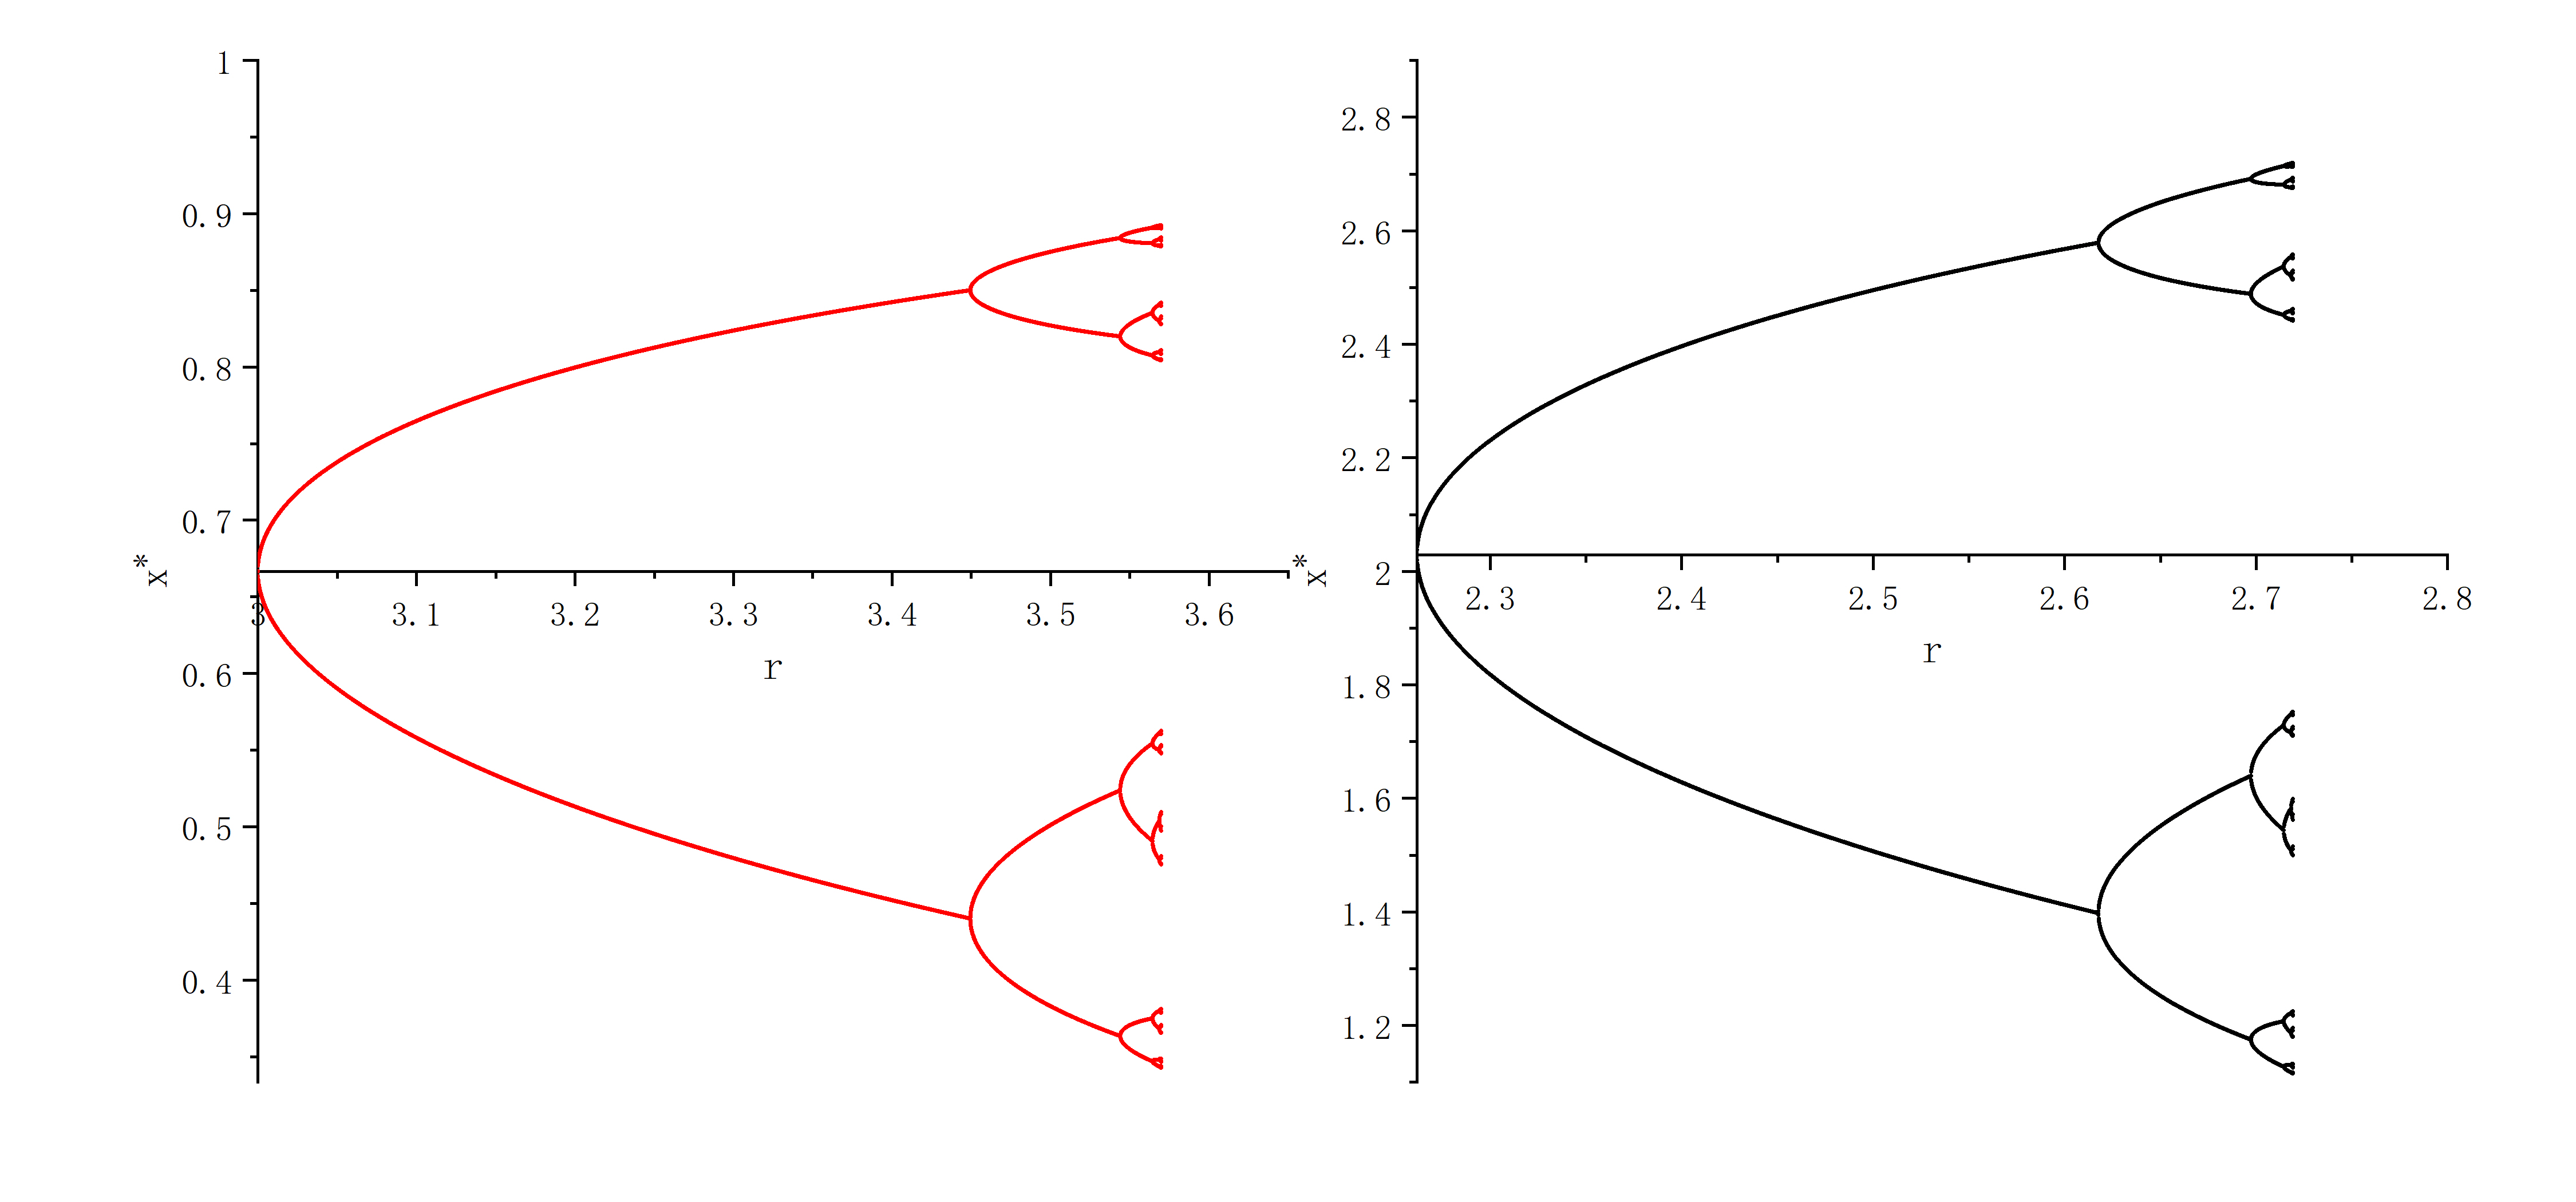
\includegraphics[width=0.8\textwidth]{x-r图对比.jpg}
        \caption{x-r图对比}
        \label{x-r图对比}
    \end{figure}

    其中左侧是第六问中的图\ref{x-r图(magnify1-2)},右侧是本问图,可以看出,二者是惊人的相似。

    \section{附录}
    \subsection{第一问源代码}
    \begin{lstlisting}[language=C]
        //本程序通过手动调整r,x,N,可以输出相应条件下的迭代序列
        #include <stdio.h>
        double r=0.5;//可调参数r
        int N=10;//迭代次数
        double x=0.1;//迭代初值
        double f(double x){
            double y=r*x*(1-x);
            return y;
        }
        int main(){
            int i;
            for ( i = 0; i < N+1; i++)
            {
                printf("%lf\n",x);
                x=f(x);
            }
            return 0;    
        }
        \end{lstlisting}

    \subsection{第五问源代码}
    \subsubsection{周期四、八展示}

        本程序需要手动调制参数r。
        \begin{lstlisting}[language=C]
            //本程序求一个r值下迭代序列第100001-100100项
            #include <stdio.h>
            #include <math.h>
            
            double r=3.55;
            long long N=100000;
            
            double f(double x){
                double y=r*x*(1-x);
                return y;
            }
            int main(){
                double x=0.9;
                long long i;
                for ( i = 0; i < N; i++)
                {
                    x=f(x);
                }
                for(i=0;i<100;i++){
                    x=f(x);
                    printf("%lf\n",x);
                } 
                return 0;
            }
        \end{lstlisting}
    \subsubsection{二分法寻找周期分点}
    \begin{lstlisting}[language=C]
        #include <stdio.h>
        #include <math.h>
        #define EPS1 1e-10//周期分点的精度
        #define EPS2 1e-16//判断数列收敛的精度
        //以下是需要手动设置的三参数
        #define A 3.4494
        #define B 3.4495
        #define N 2

        double f(double x, double r){
            double y=r*x*(1-x);
            return y;
        }
        int periodIsM(double r,int m){//对于参数r,判断序列是不是周期为m
            double x0=-9,x=0.9;//序列初值0.9,x0用于储存前一个x值
            int i;
            while ( fabs(x-x0)>EPS2){//迭代使序列收敛
                x0=x;
                for(i=0;i<2*m;i++){x=f(x,r);}
            }//由于序列周期只可能为m,m/2,2m,每隔2m取出的子序列一定收敛,
            //那么每隔2m取一个值,当与前一个值做差小于EPS2时认为序列收敛
            double y=x;
            for ( i = 0; i < m; i++){x=f(x,r);}//再迭代m次看两个值是否相近
            if(fabs(y-x)<EPS1){return 1;}//若在小于EPS1精度内相等,认为周期为m
            else return 0;
        }
        //寻找周期分点函数,原理同算法\ref{二分法求解周期分点的精确值}
        double SearchThreshold(double a, double b,int m,int n, double tol){
            if(!(periodIsM(a,m)&&periodIsM(b,n))){//区间错误
                printf("FALSE PARAMETER!\n");
                return -404404;
            }
            double r;
            while(fabs(b-a)>tol){
                r=(a+b)/2;
                if(periodIsM(r,m)){a=r;}
                else{b=r;}
            }
            return (a+b)/2;
        }
        int main(){
            double rt;
            rt=SearchThreshold(A,B,N,2*N,EPS1);
            printf("%.10lf",rt);
            return 0;
        }
    \end{lstlisting}

    \subsection{第六问源代码}
    \subsubsection{绘制V-r图}
    \begin{lstlisting}[language=C]
        #include <stdio.h>
        #include <math.h>
        #define EPS1 1e-10//原序列收敛特征长度
        #define EPS2 1e-7//收敛速度收敛特征长度

        double r=0.0001;
        double f(double x){
            double y=r*x*(1-x);
            return y;
        }
        double Nf(double x, int N){//计算序列迭代N次后的结果
            int i;
            double y=x;
            for ( i = 0; i < N; i++)
            {
                y=f(y);
            }
            return y;
        }
        int main(){//数据将输入到指定路径下的txt文件中
            FILE *fdata=fopen("C://C_files//HW1//convergentSpeed_data.txt","w");
            if (fdata==NULL)
            {
                return 0;
            }
            int i;
            while (r < 3.569892)
            {
                double x00=0.9;//$x_n$
                double x0;//$x_{n+N}$
                double x;//$x_{n+2N}$
                double V=-9,V0=-99,V00=-999,V000=-9999,V0000=-99999;
                //分别储存临近五次计算的收敛速度V
                //只有在相邻收敛速度之差都小于EPS2时,迭代才会收敛
                //|x-x0|<EPS1时被除数过小,迭代也会终止
                if(r<3){
                x0=Nf(x00,1);
                x=Nf(x0,1);
                    while(((fabs(V-V0)>EPS2)||(fabs(V0-V00)>EPS2)
                    ||(fabs(V00-V000)>EPS2)||(fabs(V000-V0000)>EPS2))
                    &&fabs(x-x0)>EPS1){
                    V0000=V000;
                    V000=V00;
                    V00=V0;
                    V0=V;
                    V=fabs((x0-x00)/(x-x0));
                    x00=x0;
                    x0=x;
                    x=Nf(x,1);
                    }
                    fprintf(fdata,"%lf %lf\n",r,V); 
                }
                else if(r<3.449490){
                    x0=Nf(x00,2);
                x=Nf(x0,2);
                    while(((fabs(V-V0)>EPS2)||(fabs(V0-V00)>EPS2)
                    ||(fabs(V00-V000)>EPS2)||(fabs(V000-V0000)>EPS2))
                    &&fabs(x-x0)>EPS1){
                    V0000=V000;
                    V000=V00;
                    V00=V0;
                    V0=V;
                    V=fabs((x0-x00)/(x-x0));
                    x00=x0;
                    x0=x;
                    x=Nf(x,2);
                    }
                    fprintf(fdata,"%lf %lf\n",r,V); 
                }
                else if(r<3.544091){
                    x0=Nf(x00,4);
                x=Nf(x0,4);
                    while(((fabs(V-V0)>EPS2)||(fabs(V0-V00)>EPS2)
                    ||(fabs(V00-V000)>EPS2)||(fabs(V000-V0000)>EPS2))
                    &&fabs(x-x0)>EPS1){
                    V0000=V000;
                    V000=V00;
                    V00=V0;
                    V0=V;
                    V=fabs((x0-x00)/(x-x0));
                    x00=x0;
                    x0=x;
                    x=Nf(x,4);
                    }
                    fprintf(fdata,"%lf %lf\n",r,V); 
                }
                else if(r<3.564408){
                    x0=Nf(x00,8);
                    x=Nf(x0,8);
                    while(((fabs(V-V0)>EPS2)||(fabs(V0-V00)>EPS2)
                    ||(fabs(V00-V000)>EPS2)||(fabs(V000-V0000)>EPS2))
                    &&fabs(x-x0)>EPS1){
                    V0000=V000;
                    V000=V00;
                    V00=V0;
                    V0=V;
                    V=fabs((x0-x00)/(x-x0));
                    x00=x0;
                    x0=x;
                    x=Nf(x,8);
                    }
                    fprintf(fdata,"%lf %lf\n",r,V); 
                }
                else if(r<3.568760){
                    x0=Nf(x00,16);
                x=Nf(x0,16);
                    while(((fabs(V-V0)>EPS2)||(fabs(V0-V00)>EPS2)
                    ||(fabs(V00-V000)>EPS2)||(fabs(V000-V0000)>EPS2))
                    &&fabs(x-x0)>EPS1){
                    V0000=V000;
                    V000=V00;
                    V00=V0;
                    V0=V;
                    V=fabs((x0-x00)/(x-x0));
                    x00=x0;
                    x0=x;
                    x=Nf(x,16);
                    }
                    fprintf(fdata,"%lf %lf\n",r,V); 
                }
                else if(r<3.569692){
                    x0=Nf(x00,32);
                x=Nf(x0,32);
                    while(((fabs(V-V0)>EPS2)||(fabs(V0-V00)>EPS2)
                    ||(fabs(V00-V000)>EPS2)||(fabs(V000-V0000)>EPS2))
                    &&fabs(x-x0)>EPS1){
                    V0000=V000;
                    V000=V00;
                    V00=V0;
                    V0=V;
                    V=fabs((x0-x00)/(x-x0));
                    x00=x0;
                    x0=x;
                    x=Nf(x,32);
                    }
                    fprintf(fdata,"%lf %lf\n",r,V); 
                }
                else if(r<3.569892){
                    x0=Nf(x00,64);
                    x=Nf(x0,64);
                    while(((fabs(V-V0)>EPS2)||(fabs(V0-V00)>EPS2)
                    ||(fabs(V00-V000)>EPS2)||(fabs(V000-V0000)>EPS2))
                    &&fabs(x-x0)>EPS1){
                    V0000=V000;
                    V000=V00;
                    V00=V0;
                    V0=V;
                    V=fabs((x0-x00)/(x-x0));
                    x00=x0;
                    x0=x;
                    x=Nf(x,64);
                    }
                    fprintf(fdata,"%lf %lf\n",r,V); 
                }
                
                if(r>3.15&&r<3.3)r+=1e-6;//部分区间取点加密
                else if(r>3.47&&x<3.52)r+=1e-6;
                else if(r>3.544)r+=1e-6;
                else r+=1e-5;
            }
            return 0;
        }
    \end{lstlisting}

    \subsubsection{绘制$x^*-r$图}
    \begin{lstlisting}[language=C]
        //本程序需要手动添加周期分点和周期数
        #include <stdio.h>
        #include <math.h>
        #define EPS 1e-10//收敛精度

        double r;
        double x;

        double f(double x){
            double y=r*x*(1-x);
            return y;
        }
        double converge(double x,int N){//迭代直到数列收敛,N为序列周期数
            double y=x;
            double y0=-9;
            int i;
            while(fabs(y-y0)>EPS){//收敛条件
                y0=y;
                for(i=0;i<N;i++){//每次迭代N次
                    y=f(y);
                }
            }
            return y;
        }
        int main(){//数据将输入到指定路径下的txt文件中
            FILE *fdata=fopen("C://C_files//HW1//question6_data.txt","w");
            if (fdata==NULL)
            {
                return 0;
            }
            int j;
            r = 0.0001;
            while (r < 3.5699)
            {
                x=0.9;
                int i=0,j;
                if(r<2.99999){
                    x=converge(x,1);//收敛后输出1个数
                fprintf(fdata,"%lf   %lf\n",r,x);
                }
                else if(r<3.4494){
                    x=converge(x,2);//收敛后输出2个数
                    for ( j = 0; j < 2; j++)
                    {
                    fprintf(fdata,"%lf   %lf\n",r,x);
                        x=f(x);
                    }
                }
                else if(r<3.5440){
                    x=converge(x,4);//收敛后输出4个数
                    for ( j = 0; j < 4; j++)
                    {
                    fprintf(fdata,"%lf   %lf\n",r,x);
                        x=f(x);
                    }
                }
                else if(r<3.5644){
                    x=converge(x,8);//收敛后输出8个数
                    for ( j = 0; j < 8; j++)
                    {
                    fprintf(fdata,"%lf   %lf\n",r,x);
                        x=f(x);
                    }
                }
                else if(r<3.5687){
                    x=converge(x,16);//收敛后输出16个数
                    for ( j = 0; j < 16; j++)
                    {
                    fprintf(fdata,"%lf   %lf\n",r,x);
                        x=f(x);
                    }
                }
                else if(r<3.5697){
                    x=converge(x,32);//收敛后输出32个数
                    for ( j = 0; j < 32; j++)
                    {
                    fprintf(fdata,"%lf   %lf\n",r,x);
                        x=f(x);
                    }
                }
                else if(r<3.5699){
                    x=converge(x,64);//收敛后输出64个数
                    for ( j = 0; j < 64; j++)
                    {
                    fprintf(fdata,"%lf   %lf\n",r,x);
                        x=f(x);
                    }
                }
                //对分点附近做出经验性的适当加细
                if(r>2.9998&&r<2.99999)r+=1e-5;
                else if(r>2.99999&&r<3)r+=1e-6;
                else if(r>3.44935&&r<3.4497)r+=1e-5;
                else r+=1e-4;
            }    
            fclose(fdata);
            return 0;
        }
    \end{lstlisting}

    \subsection{第九问源代码}
    \subsubsection{绘制V-r图}
    \begin{lstlisting}[language=C]
        #include <stdio.h>
        #include <math.h>
        #define EPS1 1e-10//原序列收敛特征长度
        #define EPS2 1e-7//收敛速度收敛特征长度
        
        double r=0.0001;
        double f(double x){
            double y=r*sin(x);
            return y;
        }
        double Nf(double x, int N){//计算序列迭代N次后的结果
            int i;
            double y=x;
            for ( i = 0; i < N; i++)
            {
                y=f(y);
            }
            return y;
        }
         int main(){//数据将输入到指定路径下的txt文件中
            FILE *fdata=fopen("C://C_files//HW1//
            convergentSpeed_Data_q9.txt","w");
            if (fdata==NULL)
            {
                return 0;
            }
            int i;
            while (r < 2.71925)
            {
                double x00=0.3;//$x_n$
                double x0;//$x_{n+N}$
                double x;//$x_{n+2N}$
                double V=-9,V0=-99,V00=-999,V000=-9999,V0000=-99999;
                //分别储存临近五次计算的收敛速度V,
                //只有在相邻收敛速度之差都小于EPS2时,迭代才会收敛
                //|x-x0|<EPS1时被除数过小,迭代也会终止
                if(r<2.26182){
                   x0=Nf(x00,1);
                   x=Nf(x0,1);
                    while(((fabs(V-V0)>EPS2)||(fabs(V0-V00)>EPS2)
                    ||(fabs(V00-V000)>EPS2)||
                    (fabs(V000-V0000)>EPS2))&&fabs(x-x0)>EPS1){
                    V0000=V000;
                    V000=V00;
                    V00=V0;
                    V0=V;
                    V=fabs((x0-x00)/(x-x0));
                    x00=x0;
                    x0=x;
                    x=Nf(x,1);
                    }
                    fprintf(fdata,"%lf %lf\n",r,V); 
                }
                else if(r<2.61778){
                    x0=Nf(x00,2);
                   x=Nf(x0,2);
                    while(((fabs(V-V0)>EPS2)||(fabs(V0-V00)>EPS2)
                    ||(fabs(V00-V000)>EPS2)||
                    (fabs(V000-V0000)>EPS2))&&fabs(x-x0)>EPS1){
                    V0000=V000;
                    V000=V00;
                    V00=V0;
                    V0=V;
                    V=fabs((x0-x00)/(x-x0));
                    x00=x0;
                    x0=x;
                    x=Nf(x,2);
                    }
                    fprintf(fdata,"%lf %lf\n",r,V); 
                }
                else if(r<2.69739){
                    x0=Nf(x00,4);
                   x=Nf(x0,4);
                    while(((fabs(V-V0)>EPS2)||(fabs(V0-V00)>EPS2)
                    ||(fabs(V00-V000)>EPS2)||
                    (fabs(V000-V0000)>EPS2))&&fabs(x-x0)>EPS1){
                    V0000=V000;
                    V000=V00;
                    V00=V0;
                    V0=V;
                    V=fabs((x0-x00)/(x-x0));
                    x00=x0;
                    x0=x;
                    x=Nf(x,4);
                    }
                    fprintf(fdata,"%lf %lf\n",r,V); 
                }
                else if(r<2.714600){
                    x0=Nf(x00,8);
                   x=Nf(x0,8);
                    while(((fabs(V-V0)>EPS2)||(fabs(V0-V00)>EPS2)
                    ||(fabs(V00-V000)>EPS2)||
                    (fabs(V000-V0000)>EPS2))&&fabs(x-x0)>EPS1){
                    V0000=V000;
                    V000=V00;
                    V00=V0;
                    V0=V;
                    V=fabs((x0-x00)/(x-x0));
                    x00=x0;
                    x0=x;
                    x=Nf(x,8);
                    }
                    fprintf(fdata,"%lf %lf\n",r,V); 
                }
                else if(r<2.718290){
                    x0=Nf(x00,16);
                   x=Nf(x0,16);
                    while(((fabs(V-V0)>EPS2)||(fabs(V0-V00)>EPS2)
                    ||(fabs(V00-V000)>EPS2)||
                    (fabs(V000-V0000)>EPS2))&&fabs(x-x0)>EPS1){
                    V0000=V000;
                    V000=V00;
                    V00=V0;
                    V0=V;
                    V=fabs((x0-x00)/(x-x0));
                    x00=x0;
                    x0=x;
                    x=Nf(x,16);
                    }
                    fprintf(fdata,"%lf %lf\n",r,V); 
                }
                else if(r<2.719081){
                    x0=Nf(x00,32);
                   x=Nf(x0,32);
                    while(((fabs(V-V0)>EPS2)||(fabs(V0-V00)>EPS2)
                    ||(fabs(V00-V000)>EPS2)||
                    (fabs(V000-V0000)>EPS2))&&fabs(x-x0)>EPS1){
                    V0000=V000;
                    V000=V00;
                    V00=V0;
                    V0=V;
                    V=fabs((x0-x00)/(x-x0));
                    x00=x0;
                    x0=x;
                    x=Nf(x,32);
                    }
                    fprintf(fdata,"%lf %lf\n",r,V); 
                }
                else if(r<2.71925){
                    x0=Nf(x00,64);
                   x=Nf(x0,64);
                    while(((fabs(V-V0)>EPS2)||(fabs(V0-V00)>EPS2)
                    ||(fabs(V00-V000)>EPS2)||
                    (fabs(V000-V0000)>EPS2))&&fabs(x-x0)>EPS1){
                    V0000=V000;
                    V000=V00;
                    V00=V0;
                    V0=V;
                    V=fabs((x0-x00)/(x-x0));
                    x00=x0;
                    x0=x;
                    x=Nf(x,64);
                    }
                    fprintf(fdata,"%lf %lf\n",r,V); 
                }
                
                if(r>2.61778)r+=1e-6;
                else r+=1e-5;
            }
            return 0;
         }
    \end{lstlisting}
    \subsubsection{绘制x-r图}
    \begin{lstlisting}[language=C]
        #include <stdio.h>
        #include <math.h>
        #define EPS 1e-10//收敛精度
        
        double r;
        double x;
        
        double f(double x){
            double y=r*sin(x);
            return y;
        }
        double converge(double x,int N){//迭代直到数列收敛,N为序列周期数
            double y=x;
            double y0=-9;
            int i;
            while(fabs(y-y0)>EPS){//收敛条件
                y0=y;
                for(i=0;i<N;i++){//每次迭代N次
                    y=f(y);
                }
            }
            return y;
        }
        int main(){//数据将输入到指定路径下的txt文件中
            FILE *fdata=fopen("C://C_files//HW1//x_r_data_q9.txt","w");
            if (fdata==NULL)
            {
                return 0;
            }
            int j;
            r = 0.0001;
            while (r < 2.71925)
            {
                x=0.9;
                int i=0,j;
                if(r<2.2618){
                    x=converge(x,1);//收敛后输出1个数
                   fprintf(fdata,"%lf   %lf\n",r,x);
                }
                else if(r<2.6178){
                    x=converge(x,2);//收敛后输出2个数
                    for ( j = 0; j < 2; j++)
                    {
                       fprintf(fdata,"%lf   %lf\n",r,x);
                        x=f(x);
                    }
                }
                else if(r<2.6974){
                    x=converge(x,4);//收敛后输出4个数
                    for ( j = 0; j < 4; j++)
                    {
                       fprintf(fdata,"%lf   %lf\n",r,x);
                        x=f(x);
                    }
                }
                else if(r<2.7146){
                    x=converge(x,8);//收敛后输出8个数
                    for ( j = 0; j < 8; j++)
                    {
                       fprintf(fdata,"%lf   %lf\n",r,x);
                        x=f(x);
                    }
                }
                else if(r<2.7183){
                    x=converge(x,16);//收敛后输出16个数
                    for ( j = 0; j < 16; j++)
                    {
                       fprintf(fdata,"%lf   %lf\n",r,x);
                        x=f(x);
                    }
                }
                else if(r<2.7191){
                    x=converge(x,32);//收敛后输出32个数
                    for ( j = 0; j < 32; j++)
                    {
                       fprintf(fdata,"%lf   %lf\n",r,x);
                        x=f(x);
                    }
                }
                else if(r<2.7193){
                    x=converge(x,64);//收敛后输出64个数
                    for ( j = 0; j < 64; j++)
                    {
                       fprintf(fdata,"%lf   %lf\n",r,x);
                        x=f(x);
                    }
                }
                r+=1e-4;
            }    
            fclose(fdata);
            return 0;
        }
        
        
    \end{lstlisting}

\end{document}